\documentclass[twoside]{book}

% Packages required by doxygen
\usepackage{fixltx2e}
\usepackage{calc}
\usepackage{doxygen}
\usepackage[export]{adjustbox} % also loads graphicx
\usepackage{graphicx}
\usepackage[utf8]{inputenc}
\usepackage{makeidx}
\usepackage{multicol}
\usepackage{multirow}
\PassOptionsToPackage{warn}{textcomp}
\usepackage{textcomp}
\usepackage[nointegrals]{wasysym}
\usepackage[table]{xcolor}

% NLS support packages
\usepackage[spanish]{babel}
% Font selection
\usepackage[T1]{fontenc}
\usepackage[scaled=.90]{helvet}
\usepackage{courier}
\usepackage{amssymb}
\usepackage{sectsty}
\renewcommand{\familydefault}{\sfdefault}
\allsectionsfont{%
  \fontseries{bc}\selectfont%
  \color{darkgray}%
}
\renewcommand{\DoxyLabelFont}{%
  \fontseries{bc}\selectfont%
  \color{darkgray}%
}
\newcommand{\+}{\discretionary{\mbox{\scriptsize$\hookleftarrow$}}{}{}}

% Page & text layout
\usepackage{geometry}
\geometry{%
  a4paper,%
  top=2.5cm,%
  bottom=2.5cm,%
  left=2.5cm,%
  right=2.5cm%
}
\tolerance=750
\hfuzz=15pt
\hbadness=750
\setlength{\emergencystretch}{15pt}
\setlength{\parindent}{0cm}
\setlength{\parskip}{3ex plus 2ex minus 2ex}
\makeatletter
\renewcommand{\paragraph}{%
  \@startsection{paragraph}{4}{0ex}{-1.0ex}{1.0ex}{%
    \normalfont\normalsize\bfseries\SS@parafont%
  }%
}
\renewcommand{\subparagraph}{%
  \@startsection{subparagraph}{5}{0ex}{-1.0ex}{1.0ex}{%
    \normalfont\normalsize\bfseries\SS@subparafont%
  }%
}
\makeatother

% Headers & footers
\usepackage{fancyhdr}
\pagestyle{fancyplain}
\fancyhead[LE]{\fancyplain{}{\bfseries\thepage}}
\fancyhead[CE]{\fancyplain{}{}}
\fancyhead[RE]{\fancyplain{}{\bfseries\leftmark}}
\fancyhead[LO]{\fancyplain{}{\bfseries\rightmark}}
\fancyhead[CO]{\fancyplain{}{}}
\fancyhead[RO]{\fancyplain{}{\bfseries\thepage}}
\fancyfoot[LE]{\fancyplain{}{}}
\fancyfoot[CE]{\fancyplain{}{}}
\fancyfoot[RE]{\fancyplain{}{\bfseries\scriptsize Generado por Doxygen }}
\fancyfoot[LO]{\fancyplain{}{\bfseries\scriptsize Generado por Doxygen }}
\fancyfoot[CO]{\fancyplain{}{}}
\fancyfoot[RO]{\fancyplain{}{}}
\renewcommand{\footrulewidth}{0.4pt}
\renewcommand{\chaptermark}[1]{%
  \markboth{#1}{}%
}
\renewcommand{\sectionmark}[1]{%
  \markright{\thesection\ #1}%
}

% Indices & bibliography
\usepackage{natbib}
\usepackage[titles]{tocloft}
\setcounter{tocdepth}{3}
\setcounter{secnumdepth}{5}
\makeindex

% Hyperlinks (required, but should be loaded last)
\usepackage{ifpdf}
\ifpdf
  \usepackage[pdftex,pagebackref=true]{hyperref}
\else
  \usepackage[ps2pdf,pagebackref=true]{hyperref}
\fi
\hypersetup{%
  colorlinks=true,%
  linkcolor=blue,%
  citecolor=blue,%
  unicode%
}

% Custom commands
\newcommand{\clearemptydoublepage}{%
  \newpage{\pagestyle{empty}\cleardoublepage}%
}

\usepackage{caption}
\captionsetup{labelsep=space,justification=centering,font={bf},singlelinecheck=off,skip=4pt,position=top}

%===== C O N T E N T S =====

\begin{document}

% Titlepage & ToC
\hypersetup{pageanchor=false,
             bookmarksnumbered=true,
             pdfencoding=unicode
            }
\pagenumbering{alph}
\begin{titlepage}
\vspace*{7cm}
\begin{center}%
{\Large My Project }\\
\vspace*{1cm}
{\large Generado por Doxygen 1.8.13}\\
\end{center}
\end{titlepage}
\clearemptydoublepage
\pagenumbering{roman}
\tableofcontents
\clearemptydoublepage
\pagenumbering{arabic}
\hypersetup{pageanchor=true}

%--- Begin generated contents ---
\chapter{Página principal}
\label{index}\hypertarget{index}{}Se demuestra como se implemento el patron de diseño Abstract para poder crear los objetos ya implementados anteriormente


\begin{DoxyItemize}
\item Haciendo uso de Open\+GL
\item Incluyendo las librerias de nuestros objetos para poer realizar estos graficos.
\item Patrones de diseño (Abstract Factory, Flyweight, Factory Method, Builder) 
\end{DoxyItemize}
\chapter{Indice jerárquico}
\section{Jerarquía de la clase}
Esta lista de herencias esta ordenada aproximadamente por orden alfabético\+:\begin{DoxyCompactList}
\item \contentsline{section}{Abstract\+Fact}{\pageref{classAbstractFact}}{}
\begin{DoxyCompactList}
\item \contentsline{section}{Prim}{\pageref{classPrim}}{}
\item \contentsline{section}{Seco}{\pageref{classSeco}}{}
\end{DoxyCompactList}
\item \contentsline{section}{caretaker}{\pageref{classcaretaker}}{}
\item \contentsline{section}{Coord}{\pageref{structCoord}}{}
\item \contentsline{section}{d\+\_\+node$<$ T $>$}{\pageref{classd__node}}{}
\item \contentsline{section}{d\+\_\+node$<$ memento $\ast$$>$}{\pageref{classd__node}}{}
\item \contentsline{section}{Director}{\pageref{classDirector}}{}
\item \contentsline{section}{double\+\_\+linked\+\_\+list$<$ T $>$}{\pageref{classdouble__linked__list}}{}
\item \contentsline{section}{double\+\_\+linked\+\_\+list$<$ memento $\ast$$>$}{\pageref{classdouble__linked__list}}{}
\item \contentsline{section}{Flower}{\pageref{classFlower}}{}
\begin{DoxyCompactList}
\item \contentsline{section}{Flor\+Bonita}{\pageref{classFlorBonita}}{}
\item \contentsline{section}{Flor\+Mala}{\pageref{classFlorMala}}{}
\item \contentsline{section}{Flor\+Normal}{\pageref{classFlorNormal}}{}
\end{DoxyCompactList}
\item \contentsline{section}{foto}{\pageref{classfoto}}{}
\item \contentsline{section}{Hoja}{\pageref{classHoja}}{}
\item \contentsline{section}{linked\+\_\+list$<$ T $>$\+:\+:iterator}{\pageref{classlinked__list_1_1iterator}}{}
\item \contentsline{section}{linked\+\_\+list$<$ T $>$}{\pageref{classlinked__list}}{}
\item \contentsline{section}{memento}{\pageref{classmemento}}{}
\item \contentsline{section}{node$<$ T $>$}{\pageref{classnode}}{}
\item \contentsline{section}{Particle}{\pageref{classParticle}}{}
\item \contentsline{section}{Rama}{\pageref{classRama}}{}
\item \contentsline{section}{Snow}{\pageref{classSnow}}{}
\item \contentsline{section}{Snow\+Fly}{\pageref{classSnowFly}}{}
\item \contentsline{section}{Tree}{\pageref{classTree}}{}
\item \contentsline{section}{Tree\+Buil}{\pageref{classTreeBuil}}{}
\begin{DoxyCompactList}
\item \contentsline{section}{Normal\+Tree}{\pageref{classNormalTree}}{}
\end{DoxyCompactList}
\item \contentsline{section}{Tronco}{\pageref{classTronco}}{}
\item \contentsline{section}{Turtle}{\pageref{classTurtle}}{}
\end{DoxyCompactList}

\chapter{Índice de clases}
\section{Lista de clases}
Lista de las clases, estructuras, uniones e interfaces con una breve descripción\+:\begin{DoxyCompactList}
\item\contentsline{section}{\hyperlink{classAbstractFact}{Abstract\+Fact} \\*La clase \hyperlink{classAbstractFact}{Abstract\+Fact} contiene funciones virtual-\/pura  Se realiza con funciones virtual-\/pura para que estas sean reutilizadas por nuestras fabricas }{\pageref{classAbstractFact}}{}
\item\contentsline{section}{\hyperlink{classcaretaker}{caretaker} }{\pageref{classcaretaker}}{}
\item\contentsline{section}{\hyperlink{structCoord}{Coord} }{\pageref{structCoord}}{}
\item\contentsline{section}{\hyperlink{classd__node}{d\+\_\+node$<$ T $>$} }{\pageref{classd__node}}{}
\item\contentsline{section}{\hyperlink{classDirector}{Director} \\*La clase \hyperlink{classDirector}{Director} cse encarga de recolectar todas las caracteristicas para poder formal lo pedido  Utilizando punteros al arbol, se logra enviar la informacion para su elaboracion }{\pageref{classDirector}}{}
\item\contentsline{section}{\hyperlink{classdouble__linked__list}{double\+\_\+linked\+\_\+list$<$ T $>$} }{\pageref{classdouble__linked__list}}{}
\item\contentsline{section}{\hyperlink{classFlorBonita}{Flor\+Bonita} \\*La clase \hyperlink{classFlorBonita}{Flor\+Bonita} contiene la funcion drawn para poder visualizarlo, hereda de la clase \hyperlink{classFlower}{Flower}  Se tiene constructor y destructor }{\pageref{classFlorBonita}}{}
\item\contentsline{section}{\hyperlink{classFlorMala}{Flor\+Mala} \\*La clase \hyperlink{classFlorMala}{Flor\+Mala} contiene tla funcion drawn para poder visualizarlo, hereda de la clase \hyperlink{classFlower}{Flower}  Se instancia el dato miembro }{\pageref{classFlorMala}}{}
\item\contentsline{section}{\hyperlink{classFlorNormal}{Flor\+Normal} \\*La clase \hyperlink{classFlorNormal}{Flor\+Normal} contiene tla funcion drawn para poder visualizarlo, hereda de la clase \hyperlink{classFlower}{Flower}  Se instancia el dato miembro }{\pageref{classFlorNormal}}{}
\item\contentsline{section}{\hyperlink{classFlower}{Flower} \\*La clase \hyperlink{classFlower}{Flower} contiene la funcion drawn para poder visualizarlo  Se instancia el dato miembro }{\pageref{classFlower}}{}
\item\contentsline{section}{\hyperlink{classfoto}{foto} }{\pageref{classfoto}}{}
\item\contentsline{section}{\hyperlink{classHoja}{Hoja} \\*La clase \hyperlink{classHoja}{Hoja} contiene la funcion drawn para poder visualizarlo  Se instancia el dato miembro }{\pageref{classHoja}}{}
\item\contentsline{section}{\hyperlink{classlinked__list_1_1iterator}{linked\+\_\+list$<$ T $>$\+::iterator} }{\pageref{classlinked__list_1_1iterator}}{}
\item\contentsline{section}{\hyperlink{classlinked__list}{linked\+\_\+list$<$ T $>$} }{\pageref{classlinked__list}}{}
\item\contentsline{section}{\hyperlink{classmemento}{memento} }{\pageref{classmemento}}{}
\item\contentsline{section}{\hyperlink{classnode}{node$<$ T $>$} }{\pageref{classnode}}{}
\item\contentsline{section}{\hyperlink{classNormalTree}{Normal\+Tree} \\*La clase \hyperlink{classNormalTree}{Normal\+Tree} contiene las funciones get\+Tronco, get\+Hojas, get\+Ramas; asi como loset sets de estas para obtener y generar las caracteristicas del arbol  Las funciones apuntan a las clases de las partes del arbol, asi como tambien son void }{\pageref{classNormalTree}}{}
\item\contentsline{section}{\hyperlink{classParticle}{Particle} \\*La clase \hyperlink{classParticle}{Particle} contiene las funciones display para poder visualizarlo, set cant y gv  Se instancia el dato miembro para cantidad y gv para los pixels que recorre por iteracion }{\pageref{classParticle}}{}
\item\contentsline{section}{\hyperlink{classPrim}{Prim} \\*La clase \hyperlink{classPrim}{Prim} es la clase \hyperlink{classAbstractFact}{Abstract\+Fact} concreta  Se instancian punteros a cada uno de nuestros objetos }{\pageref{classPrim}}{}
\item\contentsline{section}{\hyperlink{classRama}{Rama} \\*La clase \hyperlink{classRama}{Rama} contiene la funcion drawn para poder visualizarlo  Se instancia el dato miembro }{\pageref{classRama}}{}
\item\contentsline{section}{\hyperlink{classSeco}{Seco} \\*La clase \hyperlink{classSeco}{Seco} es la clase \hyperlink{classAbstractFact}{Abstract\+Fact} concreta  Se instancian punteros a cada uno de nuestros objetos pero esta vez de otro tipo }{\pageref{classSeco}}{}
\item\contentsline{section}{\hyperlink{classSnow}{Snow} \\*La clase \hyperlink{classSnow}{Snow} contiene las funciones display para poder visualizarlo, set cant y gv  Se instancia el dato miembro para cantidad, gv para los pixels que recorre por iteracion, un vector de particulas para guardar las que son pedidas por el usuario }{\pageref{classSnow}}{}
\item\contentsline{section}{\hyperlink{classSnowFly}{Snow\+Fly} \\*La clase \hyperlink{classSnowFly}{Snow\+Fly} contiene las funciones set\+Tam y get\+Tam para poder darle tamano a nuesta nieve  Se instancia el dato miembro tam }{\pageref{classSnowFly}}{}
\item\contentsline{section}{\hyperlink{classTree}{Tree} \\*La clase \hyperlink{classTree}{Tree} contiene la funcion drawn para visualizar el arbol  Se instancia los datos miembros que son punteros a las partes del arbol }{\pageref{classTree}}{}
\item\contentsline{section}{\hyperlink{classTreeBuil}{Tree\+Buil} \\*La interfaz \hyperlink{classTreeBuil}{Tree\+Buil} contiene las funciones get\+Tronco, get\+Hojas, get\+Ramas para obtener las caracteristicas del arbol  Las funciones son virtual-\/puras y apuntan a las clases de las partes del arbol }{\pageref{classTreeBuil}}{}
\item\contentsline{section}{\hyperlink{classTronco}{Tronco} \\*La clase \hyperlink{classTronco}{Tronco} contiene la funcion drawn para poder visualizarlo  Se instancia el dato miembro }{\pageref{classTronco}}{}
\item\contentsline{section}{\hyperlink{classTurtle}{Turtle} \\*La clase tortuga contiene todos los metodos y funciones de \char`\"{}turtle\char`\"{} de Python  Una numeracion general sobre los metodos mas importantes de \char`\"{}turle\char`\"{} }{\pageref{classTurtle}}{}
\end{DoxyCompactList}

\chapter{Indice de archivos}
\section{Lista de archivos}
Lista de todos los archivos documentados y con descripciones breves\+:\begin{DoxyCompactList}
\item\contentsline{section}{\hyperlink{Abstract_8h}{Abstract.\+h} \\*Implementacion de la clase \hyperlink{classAbstractFact}{Abstract\+Fact} con el uso de Open\+Gl en C++ }{\pageref{Abstract_8h}}{}
\item\contentsline{section}{\hyperlink{ArbolBuilder_8h}{Arbol\+Builder.\+h} \\*Implementacion de la clase \hyperlink{classTreeBuil}{Tree\+Buil} con el uso de Open\+Gl en C++ }{\pageref{ArbolBuilder_8h}}{}
\item\contentsline{section}{{\bfseries Caretaker.\+h} }{\pageref{Caretaker_8h}}{}
\item\contentsline{section}{\hyperlink{FlorFactoryM_8h}{Flor\+Factory\+M.\+h} \\*Implementacion de la clase \hyperlink{classFlower}{Flower} con el uso de Open\+Gl en C++ }{\pageref{FlorFactoryM_8h}}{}
\item\contentsline{section}{\hyperlink{PartiFlyweight_8h}{Parti\+Flyweight.\+h} \\*Implementacion de la clase \hyperlink{classSnowFly}{Snow\+Fly} con el uso de Open\+Gl en C++ }{\pageref{PartiFlyweight_8h}}{}
\item\contentsline{section}{\hyperlink{Turtle_8h}{Turtle.\+h} \\*Implementacion de la clase \hyperlink{classTurtle}{Turtle} con el uso de Open\+Gl en C++ }{\pageref{Turtle_8h}}{}
\end{DoxyCompactList}

\chapter{Documentación de las clases}
\hypertarget{classAbstractFact}{}\section{Referencia de la Clase Abstract\+Fact}
\label{classAbstractFact}\index{Abstract\+Fact@{Abstract\+Fact}}


La clase \hyperlink{classAbstractFact}{Abstract\+Fact} contiene funciones virtual-\/pura  Se realiza con funciones virtual-\/pura para que estas sean reutilizadas por nuestras fabricas.  




{\ttfamily \#include $<$Abstract.\+h$>$}



Diagrama de herencias de Abstract\+Fact
\nopagebreak
\begin{figure}[H]
\begin{center}
\leavevmode
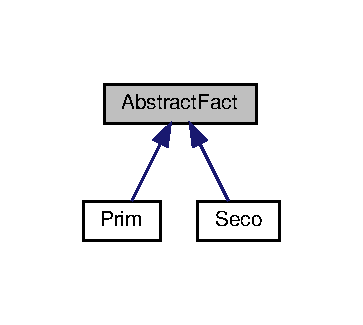
\includegraphics[width=174pt]{classAbstractFact__inherit__graph}
\end{center}
\end{figure}
\subsection*{Métodos públicos}
\begin{DoxyCompactItemize}
\item 
virtual \hyperlink{classTree}{Tree} $\ast$ \hyperlink{classAbstractFact_a37e763c0a454db79c61f229d33b72c73}{get\+Tree} ()=0
\item 
virtual \hyperlink{classFlower}{Flower} $\ast$ \hyperlink{classAbstractFact_a9ee9f34bc189886b24e325ff2412a1d9}{get\+Flor} ()=0
\item 
virtual \hyperlink{classSnow}{Snow} $\ast$ \hyperlink{classAbstractFact_a7b642a7fe5615f7103dd7d1ab4c801d9}{get\+Parti} ()=0
\end{DoxyCompactItemize}


\subsection{Descripción detallada}
La clase \hyperlink{classAbstractFact}{Abstract\+Fact} contiene funciones virtual-\/pura  Se realiza con funciones virtual-\/pura para que estas sean reutilizadas por nuestras fabricas. 

\subsection{Documentación de las funciones miembro}
\mbox{\Hypertarget{classAbstractFact_a9ee9f34bc189886b24e325ff2412a1d9}\label{classAbstractFact_a9ee9f34bc189886b24e325ff2412a1d9}} 
\index{Abstract\+Fact@{Abstract\+Fact}!get\+Flor@{get\+Flor}}
\index{get\+Flor@{get\+Flor}!Abstract\+Fact@{Abstract\+Fact}}
\subsubsection{\texorpdfstring{get\+Flor()}{getFlor()}}
{\footnotesize\ttfamily virtual \hyperlink{classFlower}{Flower}$\ast$ Abstract\+Fact\+::get\+Flor (\begin{DoxyParamCaption}{ }\end{DoxyParamCaption})\hspace{0.3cm}{\ttfamily [pure virtual]}}

Funcion virtual para poder generar nuestra flor. 

Implementado en \hyperlink{classSeco_a91092401b16231a926255323e89c6412}{Seco} y \hyperlink{classPrim_a92e3d118382a67173d008d5d82e4798c}{Prim}.

\mbox{\Hypertarget{classAbstractFact_a7b642a7fe5615f7103dd7d1ab4c801d9}\label{classAbstractFact_a7b642a7fe5615f7103dd7d1ab4c801d9}} 
\index{Abstract\+Fact@{Abstract\+Fact}!get\+Parti@{get\+Parti}}
\index{get\+Parti@{get\+Parti}!Abstract\+Fact@{Abstract\+Fact}}
\subsubsection{\texorpdfstring{get\+Parti()}{getParti()}}
{\footnotesize\ttfamily virtual \hyperlink{classSnow}{Snow}$\ast$ Abstract\+Fact\+::get\+Parti (\begin{DoxyParamCaption}{ }\end{DoxyParamCaption})\hspace{0.3cm}{\ttfamily [pure virtual]}}

Funcion virtual para poder generar nuestra nieve. 

Implementado en \hyperlink{classSeco_acd61763141ecdb895062cdde7defa800}{Seco} y \hyperlink{classPrim_ae2c1e853547a33662bd00baff26d67f8}{Prim}.

\mbox{\Hypertarget{classAbstractFact_a37e763c0a454db79c61f229d33b72c73}\label{classAbstractFact_a37e763c0a454db79c61f229d33b72c73}} 
\index{Abstract\+Fact@{Abstract\+Fact}!get\+Tree@{get\+Tree}}
\index{get\+Tree@{get\+Tree}!Abstract\+Fact@{Abstract\+Fact}}
\subsubsection{\texorpdfstring{get\+Tree()}{getTree()}}
{\footnotesize\ttfamily virtual \hyperlink{classTree}{Tree}$\ast$ Abstract\+Fact\+::get\+Tree (\begin{DoxyParamCaption}{ }\end{DoxyParamCaption})\hspace{0.3cm}{\ttfamily [pure virtual]}}

Funcion virtual para poder generar nuestro arbol.. 

Implementado en \hyperlink{classSeco_ae4a078cccba29b3d89dcb62b6eeaa269}{Seco} y \hyperlink{classPrim_aeccbb4f2821f8bc508647e2f6dd95370}{Prim}.



La documentación para esta clase fue generada a partir del siguiente fichero\+:\begin{DoxyCompactItemize}
\item 
\hyperlink{Abstract_8h}{Abstract.\+h}\end{DoxyCompactItemize}

\hypertarget{classcaretaker}{}\section{Referencia de la Clase caretaker}
\label{classcaretaker}\index{caretaker@{caretaker}}


Diagrama de colaboración para caretaker\+:\nopagebreak
\begin{figure}[H]
\begin{center}
\leavevmode
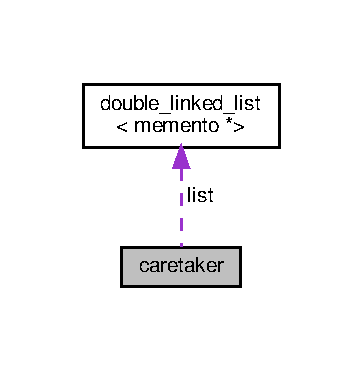
\includegraphics[width=174pt]{classcaretaker__coll__graph}
\end{center}
\end{figure}
\subsection*{Métodos públicos}
\begin{DoxyCompactItemize}
\item 
\mbox{\Hypertarget{classcaretaker_a0251f0e9f845fa596b9ce2f2beed3c71}\label{classcaretaker_a0251f0e9f845fa596b9ce2f2beed3c71}} 
void {\bfseries setmemento} (\hyperlink{classmemento}{memento} $\ast$Memento)
\item 
\mbox{\Hypertarget{classcaretaker_a1fb546ad9a4fb71eec138afb42b1a744}\label{classcaretaker_a1fb546ad9a4fb71eec138afb42b1a744}} 
\hyperlink{classmemento}{memento} $\ast$ {\bfseries getmemento} ()
\item 
\mbox{\Hypertarget{classcaretaker_aa63a4f7e099ce820998d6c7c85ec8385}\label{classcaretaker_aa63a4f7e099ce820998d6c7c85ec8385}} 
\hyperlink{classmemento}{memento} $\ast$ {\bfseries retrosede} ()
\item 
\mbox{\Hypertarget{classcaretaker_af558d2ec12cd9f95365704269ea46164}\label{classcaretaker_af558d2ec12cd9f95365704269ea46164}} 
\hyperlink{classmemento}{memento} $\ast$ {\bfseries avanzar} ()
\end{DoxyCompactItemize}
\subsection*{Atributos públicos}
\begin{DoxyCompactItemize}
\item 
\mbox{\Hypertarget{classcaretaker_ab12d0794f90bc4ef7bdecfa11f40998c}\label{classcaretaker_ab12d0794f90bc4ef7bdecfa11f40998c}} 
\hyperlink{classdouble__linked__list}{double\+\_\+linked\+\_\+list}$<$ \hyperlink{classmemento}{memento} $\ast$ $>$ {\bfseries list}
\end{DoxyCompactItemize}


La documentación para esta clase fue generada a partir del siguiente fichero\+:\begin{DoxyCompactItemize}
\item 
Caretaker.\+h\end{DoxyCompactItemize}

\hypertarget{structCoord}{}\section{Referencia de la Estructura Coord}
\label{structCoord}\index{Coord@{Coord}}
\subsection*{Métodos públicos}
\begin{DoxyCompactItemize}
\item 
\hyperlink{structCoord_add896c4f3fb15b4ad762b5270855345c}{Coord} ()
\end{DoxyCompactItemize}
\subsection*{Atributos públicos}
\begin{DoxyCompactItemize}
\item 
\mbox{\Hypertarget{structCoord_a0172a22ee75843a96e3a84ebc25f3de7}\label{structCoord_a0172a22ee75843a96e3a84ebc25f3de7}} 
double {\bfseries x}
\item 
\mbox{\Hypertarget{structCoord_af6e543e0522076e717bae53102655b87}\label{structCoord_af6e543e0522076e717bae53102655b87}} 
double {\bfseries y}
\item 
\mbox{\Hypertarget{structCoord_a8ead39d3c60427e2d428a15bfbd9b4d7}\label{structCoord_a8ead39d3c60427e2d428a15bfbd9b4d7}} 
int {\bfseries R}
\item 
\mbox{\Hypertarget{structCoord_ae23b32f330c7da521781e27f23341dae}\label{structCoord_ae23b32f330c7da521781e27f23341dae}} 
int {\bfseries G}
\item 
\mbox{\Hypertarget{structCoord_a178fbef489d3631b6f7e68f421cfec37}\label{structCoord_a178fbef489d3631b6f7e68f421cfec37}} 
int {\bfseries B}
\item 
\mbox{\Hypertarget{structCoord_a1f17c799bd8f733668e637dd706013d9}\label{structCoord_a1f17c799bd8f733668e637dd706013d9}} 
float {\bfseries de}
\end{DoxyCompactItemize}


\subsection{Documentación del constructor y destructor}
\mbox{\Hypertarget{structCoord_add896c4f3fb15b4ad762b5270855345c}\label{structCoord_add896c4f3fb15b4ad762b5270855345c}} 
\index{Coord@{Coord}!Coord@{Coord}}
\index{Coord@{Coord}!Coord@{Coord}}
\subsubsection{\texorpdfstring{Coord()}{Coord()}}
{\footnotesize\ttfamily Coord\+::\+Coord (\begin{DoxyParamCaption}{ }\end{DoxyParamCaption})\hspace{0.3cm}{\ttfamily [inline]}}

Constructor de la estructura \hyperlink{structCoord}{Coord} dando valores. 

La documentación para esta estructura fue generada a partir del siguiente fichero\+:\begin{DoxyCompactItemize}
\item 
\hyperlink{Turtle_8h}{Turtle.\+h}\end{DoxyCompactItemize}

\hypertarget{classd__node}{}\section{Referencia de la plantilla de la Clase d\+\_\+node$<$ T $>$}
\label{classd__node}\index{d\+\_\+node$<$ T $>$@{d\+\_\+node$<$ T $>$}}
\subsection*{Métodos públicos}
\begin{DoxyCompactItemize}
\item 
\mbox{\Hypertarget{classd__node_abaeebcef6100d03af4ebf6bfb52e8e0f}\label{classd__node_abaeebcef6100d03af4ebf6bfb52e8e0f}} 
{\bfseries d\+\_\+node} (const T \&d, \hyperlink{classd__node}{d\+\_\+node}$<$ T $>$ $\ast$n=N\+U\+LL, \hyperlink{classd__node}{d\+\_\+node}$<$ T $>$ $\ast$p=N\+U\+LL)
\item 
\mbox{\Hypertarget{classd__node_a7846e603daf1d89268084e5be3005719}\label{classd__node_a7846e603daf1d89268084e5be3005719}} 
void {\bfseries print} ()
\end{DoxyCompactItemize}
\subsection*{Amigas}
\begin{DoxyCompactItemize}
\item 
\mbox{\Hypertarget{classd__node_a45e00b04588b8ef146ed1c10af00ae9c}\label{classd__node_a45e00b04588b8ef146ed1c10af00ae9c}} 
class {\bfseries double\+\_\+linked\+\_\+list$<$ T $>$}
\end{DoxyCompactItemize}


La documentación para esta clase fue generada a partir del siguiente fichero\+:\begin{DoxyCompactItemize}
\item 
Linked\+List.\+cpp\end{DoxyCompactItemize}

\hypertarget{classDirector}{}\section{Referencia de la Clase Director}
\label{classDirector}\index{Director@{Director}}


La clase \hyperlink{classDirector}{Director} cse encarga de recolectar todas las caracteristicas para poder formal lo pedido  Utilizando punteros al arbol, se logra enviar la informacion para su elaboracion.  




{\ttfamily \#include $<$Arbol\+Builder.\+h$>$}

\subsection*{Métodos públicos}
\begin{DoxyCompactItemize}
\item 
void \hyperlink{classDirector_a08d3ffc5c9323cc649ba603f4b2d0758}{set\+Builder} (\hyperlink{classTreeBuil}{Tree\+Buil} $\ast$new\+Builder)
\item 
\hyperlink{classTree}{Tree} $\ast$ \hyperlink{classDirector_aeffbc977843b757e6514c91c2b040074}{get\+Builder} (int a, int b, int c)
\item 
\hyperlink{classTree}{Tree} $\ast$ \hyperlink{classDirector_aa05d4a6f7847d53486824d640654a952}{get\+Tree} ()
\end{DoxyCompactItemize}


\subsection{Descripción detallada}
La clase \hyperlink{classDirector}{Director} cse encarga de recolectar todas las caracteristicas para poder formal lo pedido  Utilizando punteros al arbol, se logra enviar la informacion para su elaboracion. 

\subsection{Documentación de las funciones miembro}
\mbox{\Hypertarget{classDirector_aeffbc977843b757e6514c91c2b040074}\label{classDirector_aeffbc977843b757e6514c91c2b040074}} 
\index{Director@{Director}!get\+Builder@{get\+Builder}}
\index{get\+Builder@{get\+Builder}!Director@{Director}}
\subsubsection{\texorpdfstring{get\+Builder()}{getBuilder()}}
{\footnotesize\ttfamily \hyperlink{classTree}{Tree} $\ast$ Director\+::get\+Builder (\begin{DoxyParamCaption}\item[{int}]{a,  }\item[{int}]{b,  }\item[{int}]{c }\end{DoxyParamCaption})}

La funcion get\+Builder recibe tres tamanos para la creacion de los objetos y es un puntero a \hyperlink{classTree}{Tree}. 
\begin{DoxyParams}{Parámetros}
{\em a,b} & y c crean un arbol base de la forma ramas, tronco y hojas respectivamente. \\
\hline
\end{DoxyParams}
\mbox{\Hypertarget{classDirector_aa05d4a6f7847d53486824d640654a952}\label{classDirector_aa05d4a6f7847d53486824d640654a952}} 
\index{Director@{Director}!get\+Tree@{get\+Tree}}
\index{get\+Tree@{get\+Tree}!Director@{Director}}
\subsubsection{\texorpdfstring{get\+Tree()}{getTree()}}
{\footnotesize\ttfamily \hyperlink{classTree}{Tree} $\ast$ Director\+::get\+Tree (\begin{DoxyParamCaption}{ }\end{DoxyParamCaption})}

La funcion get\+Tree es un puntero a \hyperlink{classTree}{Tree}, la cual nos permite obtener la informacion para la creacion del arbol \mbox{\Hypertarget{classDirector_a08d3ffc5c9323cc649ba603f4b2d0758}\label{classDirector_a08d3ffc5c9323cc649ba603f4b2d0758}} 
\index{Director@{Director}!set\+Builder@{set\+Builder}}
\index{set\+Builder@{set\+Builder}!Director@{Director}}
\subsubsection{\texorpdfstring{set\+Builder()}{setBuilder()}}
{\footnotesize\ttfamily void Director\+::set\+Builder (\begin{DoxyParamCaption}\item[{\hyperlink{classTreeBuil}{Tree\+Buil} $\ast$}]{new\+Builder }\end{DoxyParamCaption})}

La funcion set\+Builder envia las caracteristicas definidas. 
\begin{DoxyParams}{Parámetros}
{\em new\+Builder} & es un puntor a Builder, para que las caracteristicas sean enviadas directamente. \\
\hline
\end{DoxyParams}


La documentación para esta clase fue generada a partir de los siguientes ficheros\+:\begin{DoxyCompactItemize}
\item 
\hyperlink{ArbolBuilder_8h}{Arbol\+Builder.\+h}\item 
Arbol\+Builder.\+cpp\end{DoxyCompactItemize}

\hypertarget{classdouble__linked__list}{}\section{Referencia de la plantilla de la Clase double\+\_\+linked\+\_\+list$<$ T $>$}
\label{classdouble__linked__list}\index{double\+\_\+linked\+\_\+list$<$ T $>$@{double\+\_\+linked\+\_\+list$<$ T $>$}}
\subsection*{Métodos públicos}
\begin{DoxyCompactItemize}
\item 
\mbox{\Hypertarget{classdouble__linked__list_a4f3ac6d969a61d5627816e32f1431be8}\label{classdouble__linked__list_a4f3ac6d969a61d5627816e32f1431be8}} 
void {\bfseries insert\+\_\+front} (const T \&d)
\item 
\mbox{\Hypertarget{classdouble__linked__list_ab1bff557b13a3efb9455b58bcb6d7f07}\label{classdouble__linked__list_ab1bff557b13a3efb9455b58bcb6d7f07}} 
void {\bfseries insert\+\_\+back} (const T \&d)
\item 
\mbox{\Hypertarget{classdouble__linked__list_a613ff6b3282f2395cbf0cec6f27f0bdf}\label{classdouble__linked__list_a613ff6b3282f2395cbf0cec6f27f0bdf}} 
void {\bfseries remove\+\_\+front} ()
\item 
\mbox{\Hypertarget{classdouble__linked__list_a260c3143d252a65b2a9349c68bfb7d01}\label{classdouble__linked__list_a260c3143d252a65b2a9349c68bfb7d01}} 
void {\bfseries remove\+\_\+back} ()
\item 
\mbox{\Hypertarget{classdouble__linked__list_a5fa1033307ab6b7b0d892c005d46ec8c}\label{classdouble__linked__list_a5fa1033307ab6b7b0d892c005d46ec8c}} 
void {\bfseries reverse} ()
\item 
\mbox{\Hypertarget{classdouble__linked__list_aa9477a4eb09a8e3330c616799afde4f2}\label{classdouble__linked__list_aa9477a4eb09a8e3330c616799afde4f2}} 
T {\bfseries Begin} ()
\item 
\mbox{\Hypertarget{classdouble__linked__list_a11ad63ed7ea02ddbe3205c6d6c4e426b}\label{classdouble__linked__list_a11ad63ed7ea02ddbe3205c6d6c4e426b}} 
T {\bfseries get\+Last\+Dato} ()
\item 
\mbox{\Hypertarget{classdouble__linked__list_a9717b04539be395c0e8e129738d5910d}\label{classdouble__linked__list_a9717b04539be395c0e8e129738d5910d}} 
T {\bfseries retroceder} ()
\item 
\mbox{\Hypertarget{classdouble__linked__list_ab41cc5b1dc2011112a70e5b50874da13}\label{classdouble__linked__list_ab41cc5b1dc2011112a70e5b50874da13}} 
T {\bfseries avanzar} ()
\item 
\mbox{\Hypertarget{classdouble__linked__list_aaaded0e7d96f67ca1652e8b3b4e2ba0b}\label{classdouble__linked__list_aaaded0e7d96f67ca1652e8b3b4e2ba0b}} 
void {\bfseries print} ()
\item 
\mbox{\Hypertarget{classdouble__linked__list_ace6c38d671f63f7ccdbe8492e01208a2}\label{classdouble__linked__list_ace6c38d671f63f7ccdbe8492e01208a2}} 
void {\bfseries \+\_\+size} (\hyperlink{classd__node}{d\+\_\+node}$<$ T $>$ $\ast$n)
\item 
\mbox{\Hypertarget{classdouble__linked__list_af445b5031cb0a7213a4ed5d4f3738fdb}\label{classdouble__linked__list_af445b5031cb0a7213a4ed5d4f3738fdb}} 
int {\bfseries size} ()
\end{DoxyCompactItemize}


La documentación para esta clase fue generada a partir del siguiente fichero\+:\begin{DoxyCompactItemize}
\item 
Linked\+List.\+cpp\end{DoxyCompactItemize}

\hypertarget{classFlorBonita}{}\section{Referencia de la Clase Flor\+Bonita}
\label{classFlorBonita}\index{Flor\+Bonita@{Flor\+Bonita}}


La clase \hyperlink{classFlorBonita}{Flor\+Bonita} contiene la funcion drawn para poder visualizarlo, hereda de la clase \hyperlink{classFlower}{Flower}  Se tiene constructor y destructor.  




{\ttfamily \#include $<$Flor\+Factory\+M.\+h$>$}



Diagrama de herencias de Flor\+Bonita\nopagebreak
\begin{figure}[H]
\begin{center}
\leavevmode
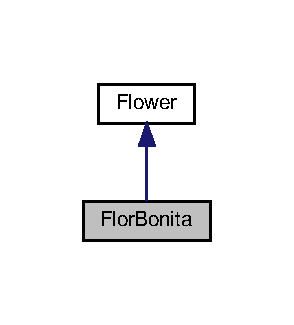
\includegraphics[width=141pt]{classFlorBonita__inherit__graph}
\end{center}
\end{figure}


Diagrama de colaboración para Flor\+Bonita\+:\nopagebreak
\begin{figure}[H]
\begin{center}
\leavevmode
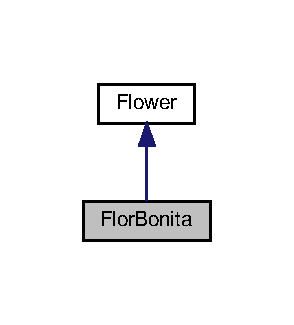
\includegraphics[width=141pt]{classFlorBonita__coll__graph}
\end{center}
\end{figure}
\subsection*{Métodos públicos}
\begin{DoxyCompactItemize}
\item 
\hyperlink{classFlorBonita_afccba3e47c8f7ad9e6da420aeba9769f}{Flor\+Bonita} (int petal)
\item 
\hyperlink{classFlorBonita_ada709e8050834cb8d988b5ba1bc558dc}{$\sim$\+Flor\+Bonita} ()
\item 
void \hyperlink{classFlorBonita_a028f32ccf00bb677f54349afa49657e4}{drawn} (\hyperlink{classTurtle}{Turtle} T, int x, int y)
\end{DoxyCompactItemize}
\subsection*{Otros miembros heredados}


\subsection{Descripción detallada}
La clase \hyperlink{classFlorBonita}{Flor\+Bonita} contiene la funcion drawn para poder visualizarlo, hereda de la clase \hyperlink{classFlower}{Flower}  Se tiene constructor y destructor. 

\subsection{Documentación del constructor y destructor}
\mbox{\Hypertarget{classFlorBonita_afccba3e47c8f7ad9e6da420aeba9769f}\label{classFlorBonita_afccba3e47c8f7ad9e6da420aeba9769f}} 
\index{Flor\+Bonita@{Flor\+Bonita}!Flor\+Bonita@{Flor\+Bonita}}
\index{Flor\+Bonita@{Flor\+Bonita}!Flor\+Bonita@{Flor\+Bonita}}
\subsubsection{\texorpdfstring{Flor\+Bonita()}{FlorBonita()}}
{\footnotesize\ttfamily Flor\+Bonita\+::\+Flor\+Bonita (\begin{DoxyParamCaption}\item[{int}]{petal }\end{DoxyParamCaption})}

Constructor. 
\begin{DoxyParams}{Parámetros}
{\em petal} & es la cantidad de petalos que tiene la flor. \\
\hline
\end{DoxyParams}
\mbox{\Hypertarget{classFlorBonita_ada709e8050834cb8d988b5ba1bc558dc}\label{classFlorBonita_ada709e8050834cb8d988b5ba1bc558dc}} 
\index{Flor\+Bonita@{Flor\+Bonita}!````~Flor\+Bonita@{$\sim$\+Flor\+Bonita}}
\index{````~Flor\+Bonita@{$\sim$\+Flor\+Bonita}!Flor\+Bonita@{Flor\+Bonita}}
\subsubsection{\texorpdfstring{$\sim$\+Flor\+Bonita()}{~FlorBonita()}}
{\footnotesize\ttfamily Flor\+Bonita\+::$\sim$\+Flor\+Bonita (\begin{DoxyParamCaption}{ }\end{DoxyParamCaption})}

Destructor 

\subsection{Documentación de las funciones miembro}
\mbox{\Hypertarget{classFlorBonita_a028f32ccf00bb677f54349afa49657e4}\label{classFlorBonita_a028f32ccf00bb677f54349afa49657e4}} 
\index{Flor\+Bonita@{Flor\+Bonita}!drawn@{drawn}}
\index{drawn@{drawn}!Flor\+Bonita@{Flor\+Bonita}}
\subsubsection{\texorpdfstring{drawn()}{drawn()}}
{\footnotesize\ttfamily void Flor\+Bonita\+::drawn (\begin{DoxyParamCaption}\item[{\hyperlink{classTurtle}{Turtle}}]{T,  }\item[{int}]{x,  }\item[{int}]{y }\end{DoxyParamCaption})\hspace{0.3cm}{\ttfamily [virtual]}}

La funcion drawn recibe la tortuga y el tamano. 
\begin{DoxyParams}{Parámetros}
{\em T,nos} & permite hacer uso de la tortuga y x, y coordinan el tamano del tronco. \\
\hline
\end{DoxyParams}


Implementa \hyperlink{classFlower_af01eea570f9d02e16cda1d86ee97633c}{Flower}.



La documentación para esta clase fue generada a partir de los siguientes ficheros\+:\begin{DoxyCompactItemize}
\item 
\hyperlink{FlorFactoryM_8h}{Flor\+Factory\+M.\+h}\item 
Flor\+Factory\+M.\+cpp\end{DoxyCompactItemize}

\hypertarget{classFlorMala}{}\section{Referencia de la Clase Flor\+Mala}
\label{classFlorMala}\index{Flor\+Mala@{Flor\+Mala}}


La clase \hyperlink{classFlorMala}{Flor\+Mala} contiene tla funcion drawn para poder visualizarlo, hereda de la clase \hyperlink{classFlower}{Flower}  Se instancia el dato miembro.  




{\ttfamily \#include $<$Flor\+Factory\+M.\+h$>$}



Diagrama de herencias de Flor\+Mala\nopagebreak
\begin{figure}[H]
\begin{center}
\leavevmode
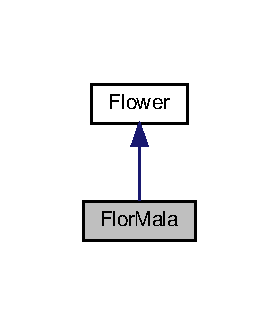
\includegraphics[width=134pt]{classFlorMala__inherit__graph}
\end{center}
\end{figure}


Diagrama de colaboración para Flor\+Mala\+:\nopagebreak
\begin{figure}[H]
\begin{center}
\leavevmode
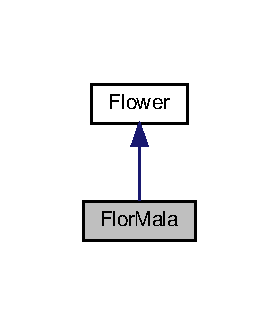
\includegraphics[width=134pt]{classFlorMala__coll__graph}
\end{center}
\end{figure}
\subsection*{Métodos públicos}
\begin{DoxyCompactItemize}
\item 
\hyperlink{classFlorMala_ae429d216656c3c4ea50e71ee0740079f}{Flor\+Mala} (int petal)
\item 
\hyperlink{classFlorMala_ae85e1a4162127aad42b44d6609e5ce3f}{$\sim$\+Flor\+Mala} ()
\item 
void \hyperlink{classFlorMala_aee0f20f3aa80d9ce3cb9c6fdbf036a7c}{drawn} (\hyperlink{classTurtle}{Turtle} T, int x, int y)
\end{DoxyCompactItemize}
\subsection*{Otros miembros heredados}


\subsection{Descripción detallada}
La clase \hyperlink{classFlorMala}{Flor\+Mala} contiene tla funcion drawn para poder visualizarlo, hereda de la clase \hyperlink{classFlower}{Flower}  Se instancia el dato miembro. 

\subsection{Documentación del constructor y destructor}
\mbox{\Hypertarget{classFlorMala_ae429d216656c3c4ea50e71ee0740079f}\label{classFlorMala_ae429d216656c3c4ea50e71ee0740079f}} 
\index{Flor\+Mala@{Flor\+Mala}!Flor\+Mala@{Flor\+Mala}}
\index{Flor\+Mala@{Flor\+Mala}!Flor\+Mala@{Flor\+Mala}}
\subsubsection{\texorpdfstring{Flor\+Mala()}{FlorMala()}}
{\footnotesize\ttfamily Flor\+Mala\+::\+Flor\+Mala (\begin{DoxyParamCaption}\item[{int}]{petal }\end{DoxyParamCaption})}

Constructor. 
\begin{DoxyParams}{Parámetros}
{\em petal} & es la cantidad de petalos que tiene la flor. \\
\hline
\end{DoxyParams}
\mbox{\Hypertarget{classFlorMala_ae85e1a4162127aad42b44d6609e5ce3f}\label{classFlorMala_ae85e1a4162127aad42b44d6609e5ce3f}} 
\index{Flor\+Mala@{Flor\+Mala}!````~Flor\+Mala@{$\sim$\+Flor\+Mala}}
\index{````~Flor\+Mala@{$\sim$\+Flor\+Mala}!Flor\+Mala@{Flor\+Mala}}
\subsubsection{\texorpdfstring{$\sim$\+Flor\+Mala()}{~FlorMala()}}
{\footnotesize\ttfamily Flor\+Mala\+::$\sim$\+Flor\+Mala (\begin{DoxyParamCaption}{ }\end{DoxyParamCaption})}

Destructor 

\subsection{Documentación de las funciones miembro}
\mbox{\Hypertarget{classFlorMala_aee0f20f3aa80d9ce3cb9c6fdbf036a7c}\label{classFlorMala_aee0f20f3aa80d9ce3cb9c6fdbf036a7c}} 
\index{Flor\+Mala@{Flor\+Mala}!drawn@{drawn}}
\index{drawn@{drawn}!Flor\+Mala@{Flor\+Mala}}
\subsubsection{\texorpdfstring{drawn()}{drawn()}}
{\footnotesize\ttfamily void Flor\+Mala\+::drawn (\begin{DoxyParamCaption}\item[{\hyperlink{classTurtle}{Turtle}}]{T,  }\item[{int}]{x,  }\item[{int}]{y }\end{DoxyParamCaption})\hspace{0.3cm}{\ttfamily [virtual]}}

La funcion drawn recibe la tortuga y el tamano. 
\begin{DoxyParams}{Parámetros}
{\em T,nos} & permite hacer uso de la tortuga y x, y coordinan el tamano del tronco. \\
\hline
\end{DoxyParams}


Implementa \hyperlink{classFlower_af01eea570f9d02e16cda1d86ee97633c}{Flower}.



La documentación para esta clase fue generada a partir de los siguientes ficheros\+:\begin{DoxyCompactItemize}
\item 
\hyperlink{FlorFactoryM_8h}{Flor\+Factory\+M.\+h}\item 
Flor\+Factory\+M.\+cpp\end{DoxyCompactItemize}

\hypertarget{classFlorNormal}{}\section{Referencia de la Clase Flor\+Normal}
\label{classFlorNormal}\index{Flor\+Normal@{Flor\+Normal}}


La clase \hyperlink{classFlorNormal}{Flor\+Normal} contiene tla funcion drawn para poder visualizarlo, hereda de la clase \hyperlink{classFlower}{Flower}  Se instancia el dato miembro.  




{\ttfamily \#include $<$Flor\+Factory\+M.\+h$>$}



Diagrama de herencias de Flor\+Normal\nopagebreak
\begin{figure}[H]
\begin{center}
\leavevmode
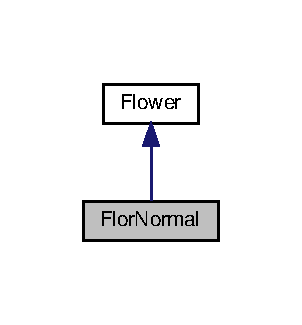
\includegraphics[width=145pt]{classFlorNormal__inherit__graph}
\end{center}
\end{figure}


Diagrama de colaboración para Flor\+Normal\+:\nopagebreak
\begin{figure}[H]
\begin{center}
\leavevmode
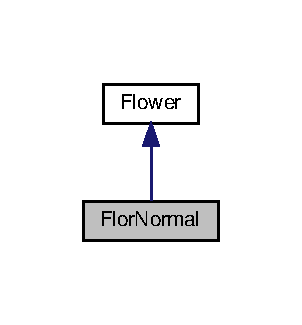
\includegraphics[width=145pt]{classFlorNormal__coll__graph}
\end{center}
\end{figure}
\subsection*{Métodos públicos}
\begin{DoxyCompactItemize}
\item 
\hyperlink{classFlorNormal_a625a13a2e2d334eceb295ef994637d25}{Flor\+Normal} (int petal)
\item 
\hyperlink{classFlorNormal_a96ed2aba6c2f54bd4312330ad1d56d42}{$\sim$\+Flor\+Normal} ()
\item 
void \hyperlink{classFlorNormal_a2e8ae341ef8bea1459baa12966eb1cd2}{drawn} (\hyperlink{classTurtle}{Turtle} p, int x, int y)
\end{DoxyCompactItemize}
\subsection*{Otros miembros heredados}


\subsection{Descripción detallada}
La clase \hyperlink{classFlorNormal}{Flor\+Normal} contiene tla funcion drawn para poder visualizarlo, hereda de la clase \hyperlink{classFlower}{Flower}  Se instancia el dato miembro. 

\subsection{Documentación del constructor y destructor}
\mbox{\Hypertarget{classFlorNormal_a625a13a2e2d334eceb295ef994637d25}\label{classFlorNormal_a625a13a2e2d334eceb295ef994637d25}} 
\index{Flor\+Normal@{Flor\+Normal}!Flor\+Normal@{Flor\+Normal}}
\index{Flor\+Normal@{Flor\+Normal}!Flor\+Normal@{Flor\+Normal}}
\subsubsection{\texorpdfstring{Flor\+Normal()}{FlorNormal()}}
{\footnotesize\ttfamily Flor\+Normal\+::\+Flor\+Normal (\begin{DoxyParamCaption}\item[{int}]{petal }\end{DoxyParamCaption})}

Constructor. 
\begin{DoxyParams}{Parámetros}
{\em petal} & es la cantidad de petalos que tiene la flor. \\
\hline
\end{DoxyParams}
\mbox{\Hypertarget{classFlorNormal_a96ed2aba6c2f54bd4312330ad1d56d42}\label{classFlorNormal_a96ed2aba6c2f54bd4312330ad1d56d42}} 
\index{Flor\+Normal@{Flor\+Normal}!````~Flor\+Normal@{$\sim$\+Flor\+Normal}}
\index{````~Flor\+Normal@{$\sim$\+Flor\+Normal}!Flor\+Normal@{Flor\+Normal}}
\subsubsection{\texorpdfstring{$\sim$\+Flor\+Normal()}{~FlorNormal()}}
{\footnotesize\ttfamily Flor\+Normal\+::$\sim$\+Flor\+Normal (\begin{DoxyParamCaption}{ }\end{DoxyParamCaption})}

Destructor 

\subsection{Documentación de las funciones miembro}
\mbox{\Hypertarget{classFlorNormal_a2e8ae341ef8bea1459baa12966eb1cd2}\label{classFlorNormal_a2e8ae341ef8bea1459baa12966eb1cd2}} 
\index{Flor\+Normal@{Flor\+Normal}!drawn@{drawn}}
\index{drawn@{drawn}!Flor\+Normal@{Flor\+Normal}}
\subsubsection{\texorpdfstring{drawn()}{drawn()}}
{\footnotesize\ttfamily void Flor\+Normal\+::drawn (\begin{DoxyParamCaption}\item[{\hyperlink{classTurtle}{Turtle}}]{p,  }\item[{int}]{x,  }\item[{int}]{y }\end{DoxyParamCaption})\hspace{0.3cm}{\ttfamily [virtual]}}

La funcion drawn recibe la tortuga y el tamano. 
\begin{DoxyParams}{Parámetros}
{\em T,nos} & permite hacer uso de la tortuga y x, y coordinan el tamano del tronco. \\
\hline
\end{DoxyParams}


Implementa \hyperlink{classFlower_af01eea570f9d02e16cda1d86ee97633c}{Flower}.



La documentación para esta clase fue generada a partir de los siguientes ficheros\+:\begin{DoxyCompactItemize}
\item 
\hyperlink{FlorFactoryM_8h}{Flor\+Factory\+M.\+h}\item 
Flor\+Factory\+M.\+cpp\end{DoxyCompactItemize}

\hypertarget{classFlower}{}\section{Referencia de la Clase Flower}
\label{classFlower}\index{Flower@{Flower}}


La clase \hyperlink{classFlower}{Flower} contiene la funcion drawn para poder visualizarlo  Se instancia el dato miembro.  




{\ttfamily \#include $<$Flor\+Factory\+M.\+h$>$}



Diagrama de herencias de Flower\nopagebreak
\begin{figure}[H]
\begin{center}
\leavevmode
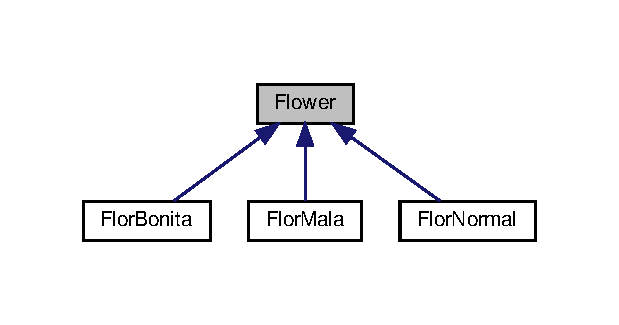
\includegraphics[width=297pt]{classFlower__inherit__graph}
\end{center}
\end{figure}
\subsection*{Métodos públicos}
\begin{DoxyCompactItemize}
\item 
virtual void \hyperlink{classFlower_af01eea570f9d02e16cda1d86ee97633c}{drawn} (\hyperlink{classTurtle}{Turtle} T, int x, int y)=0
\end{DoxyCompactItemize}
\subsection*{Atributos protegidos}
\begin{DoxyCompactItemize}
\item 
\mbox{\Hypertarget{classFlower_a219dc895fadc1d1c8850d205cae4f9a2}\label{classFlower_a219dc895fadc1d1c8850d205cae4f9a2}} 
int {\bfseries petalos}
\end{DoxyCompactItemize}


\subsection{Descripción detallada}
La clase \hyperlink{classFlower}{Flower} contiene la funcion drawn para poder visualizarlo  Se instancia el dato miembro. 

\subsection{Documentación de las funciones miembro}
\mbox{\Hypertarget{classFlower_af01eea570f9d02e16cda1d86ee97633c}\label{classFlower_af01eea570f9d02e16cda1d86ee97633c}} 
\index{Flower@{Flower}!drawn@{drawn}}
\index{drawn@{drawn}!Flower@{Flower}}
\subsubsection{\texorpdfstring{drawn()}{drawn()}}
{\footnotesize\ttfamily virtual void Flower\+::drawn (\begin{DoxyParamCaption}\item[{\hyperlink{classTurtle}{Turtle}}]{T,  }\item[{int}]{x,  }\item[{int}]{y }\end{DoxyParamCaption})\hspace{0.3cm}{\ttfamily [pure virtual]}}

Funcion para drawn. 
\begin{DoxyParams}{Parámetros}
{\em T,nos} & permite hacer uso de la tortuga y x, y coordinan el tamano del tronco \\
\hline
\end{DoxyParams}


Implementado en \hyperlink{classFlorNormal_a2e8ae341ef8bea1459baa12966eb1cd2}{Flor\+Normal}, \hyperlink{classFlorMala_aee0f20f3aa80d9ce3cb9c6fdbf036a7c}{Flor\+Mala} y \hyperlink{classFlorBonita_a028f32ccf00bb677f54349afa49657e4}{Flor\+Bonita}.



La documentación para esta clase fue generada a partir del siguiente fichero\+:\begin{DoxyCompactItemize}
\item 
\hyperlink{FlorFactoryM_8h}{Flor\+Factory\+M.\+h}\end{DoxyCompactItemize}

\hypertarget{classfoto}{}\section{Referencia de la Clase foto}
\label{classfoto}\index{foto@{foto}}
\subsection*{Métodos públicos}
\begin{DoxyCompactItemize}
\item 
\mbox{\Hypertarget{classfoto_a87c49edad87afa27208c8377d328107b}\label{classfoto_a87c49edad87afa27208c8377d328107b}} 
{\bfseries foto} (int \+\_\+state)
\item 
\mbox{\Hypertarget{classfoto_a2ceb27149200585e9455dbeb21977692}\label{classfoto_a2ceb27149200585e9455dbeb21977692}} 
void {\bfseries setmemento} (\hyperlink{classmemento}{memento} $\ast$Memento)
\item 
\mbox{\Hypertarget{classfoto_a41168a5515f628893b54d540168f1884}\label{classfoto_a41168a5515f628893b54d540168f1884}} 
\hyperlink{classmemento}{memento} $\ast$ {\bfseries creatememento} ()
\item 
\mbox{\Hypertarget{classfoto_ad57cd1e69ff6abc1a41bbb6c0ce76a7b}\label{classfoto_ad57cd1e69ff6abc1a41bbb6c0ce76a7b}} 
void {\bfseries setstate} (int \+\_\+state)
\item 
\mbox{\Hypertarget{classfoto_a9603dd12c943dce5b2a5f71af155db0b}\label{classfoto_a9603dd12c943dce5b2a5f71af155db0b}} 
int {\bfseries getstate} ()
\item 
\mbox{\Hypertarget{classfoto_a2de57a7bdc220fb3c9c191096aa6a498}\label{classfoto_a2de57a7bdc220fb3c9c191096aa6a498}} 
void {\bfseries dibujar} ()
\end{DoxyCompactItemize}


La documentación para esta clase fue generada a partir del siguiente fichero\+:\begin{DoxyCompactItemize}
\item 
Foto.\+h\end{DoxyCompactItemize}

\hypertarget{classHoja}{}\section{Referencia de la Clase Hoja}
\label{classHoja}\index{Hoja@{Hoja}}


La clase \hyperlink{classHoja}{Hoja} contiene la funcion drawn para poder visualizarlo  Se instancia el dato miembro.  




{\ttfamily \#include $<$Arbol\+Builder.\+h$>$}

\subsection*{Métodos públicos}
\begin{DoxyCompactItemize}
\item 
void \hyperlink{classHoja_aa870a3c3140e05a139d0293c3e9ca426}{drawn} (\hyperlink{classTurtle}{Turtle} T, int x, int y)
\end{DoxyCompactItemize}
\subsection*{Atributos públicos}
\begin{DoxyCompactItemize}
\item 
\mbox{\Hypertarget{classHoja_aebe2199a9f2c6774d3cbd51493ca67d6}\label{classHoja_aebe2199a9f2c6774d3cbd51493ca67d6}} 
int {\bfseries size}
\end{DoxyCompactItemize}


\subsection{Descripción detallada}
La clase \hyperlink{classHoja}{Hoja} contiene la funcion drawn para poder visualizarlo  Se instancia el dato miembro. 

\subsection{Documentación de las funciones miembro}
\mbox{\Hypertarget{classHoja_aa870a3c3140e05a139d0293c3e9ca426}\label{classHoja_aa870a3c3140e05a139d0293c3e9ca426}} 
\index{Hoja@{Hoja}!drawn@{drawn}}
\index{drawn@{drawn}!Hoja@{Hoja}}
\subsubsection{\texorpdfstring{drawn()}{drawn()}}
{\footnotesize\ttfamily void Hoja\+::drawn (\begin{DoxyParamCaption}\item[{\hyperlink{classTurtle}{Turtle}}]{T,  }\item[{int}]{x,  }\item[{int}]{y }\end{DoxyParamCaption})}

La funcion drawn recibe la tortuga y el tamano. 
\begin{DoxyParams}{Parámetros}
{\em T,nos} & permite hacer uso de la tortuga y x, y coordinan el tamano de la hoja. \\
\hline
\end{DoxyParams}


La documentación para esta clase fue generada a partir de los siguientes ficheros\+:\begin{DoxyCompactItemize}
\item 
\hyperlink{ArbolBuilder_8h}{Arbol\+Builder.\+h}\item 
Arbol\+Builder.\+cpp\end{DoxyCompactItemize}

\hypertarget{classlinked__list_1_1iterator}{}\section{Referencia de la Clase linked\+\_\+list$<$ T $>$\+:\+:iterator}
\label{classlinked__list_1_1iterator}\index{linked\+\_\+list$<$ T $>$\+::iterator@{linked\+\_\+list$<$ T $>$\+::iterator}}
\subsection*{Métodos públicos}
\begin{DoxyCompactItemize}
\item 
\mbox{\Hypertarget{classlinked__list_1_1iterator_a509f40c4aace70c08014bcf7c31a3c9a}\label{classlinked__list_1_1iterator_a509f40c4aace70c08014bcf7c31a3c9a}} 
{\bfseries iterator} (\hyperlink{classnode}{node}$<$ T $>$ $\ast$\+\_\+n)
\item 
\mbox{\Hypertarget{classlinked__list_1_1iterator_afde8572a561e469f96a23e91acdc501c}\label{classlinked__list_1_1iterator_afde8572a561e469f96a23e91acdc501c}} 
\hyperlink{classlinked__list_1_1iterator}{iterator} \& {\bfseries operator++} ()
\item 
\mbox{\Hypertarget{classlinked__list_1_1iterator_aef0f06b8677cedceaa3e709fbc5f65cb}\label{classlinked__list_1_1iterator_aef0f06b8677cedceaa3e709fbc5f65cb}} 
bool {\bfseries operator!=} (const \hyperlink{classlinked__list_1_1iterator}{iterator} \&it)
\item 
\mbox{\Hypertarget{classlinked__list_1_1iterator_ab6f6fa8309ba57362dbc37f6f3e605db}\label{classlinked__list_1_1iterator_ab6f6fa8309ba57362dbc37f6f3e605db}} 
const T \& {\bfseries operator$\ast$} ()
\end{DoxyCompactItemize}


La documentación para esta clase fue generada a partir del siguiente fichero\+:\begin{DoxyCompactItemize}
\item 
Linked\+List..\+h\end{DoxyCompactItemize}

\hypertarget{classlinked__list}{}\section{Referencia de la plantilla de la Clase linked\+\_\+list$<$ T $>$}
\label{classlinked__list}\index{linked\+\_\+list$<$ T $>$@{linked\+\_\+list$<$ T $>$}}
\subsection*{Clases}
\begin{DoxyCompactItemize}
\item 
class \hyperlink{classlinked__list_1_1iterator}{iterator}
\end{DoxyCompactItemize}
\subsection*{Métodos públicos}
\begin{DoxyCompactItemize}
\item 
\mbox{\Hypertarget{classlinked__list_afcf41d312092d12c91600b8290b03f06}\label{classlinked__list_afcf41d312092d12c91600b8290b03f06}} 
void {\bfseries insert\+\_\+front} (const T \&d)
\item 
\mbox{\Hypertarget{classlinked__list_a1f681f456c1825bf1f62e51d7bc23da4}\label{classlinked__list_a1f681f456c1825bf1f62e51d7bc23da4}} 
void {\bfseries insert\+\_\+back} (const T \&d)
\item 
\mbox{\Hypertarget{classlinked__list_a75f6a9a14e0fe46510927a7f48b30501}\label{classlinked__list_a75f6a9a14e0fe46510927a7f48b30501}} 
bool {\bfseries find} (const T \&d)
\item 
\mbox{\Hypertarget{classlinked__list_af04f395763ffbbd45500a4f10783dae0}\label{classlinked__list_af04f395763ffbbd45500a4f10783dae0}} 
void {\bfseries remove\+\_\+front} ()
\item 
\mbox{\Hypertarget{classlinked__list_ab318cceadb4d06f564a7ac7caae0c905}\label{classlinked__list_ab318cceadb4d06f564a7ac7caae0c905}} 
void {\bfseries remove\+\_\+back} ()
\item 
\mbox{\Hypertarget{classlinked__list_a15bc074e7cee3245e603ce2e136c65e1}\label{classlinked__list_a15bc074e7cee3245e603ce2e136c65e1}} 
void {\bfseries reverse} ()
\item 
\mbox{\Hypertarget{classlinked__list_a4e62feaa58fccb8a00544cd77634301c}\label{classlinked__list_a4e62feaa58fccb8a00544cd77634301c}} 
T {\bfseries get\+First\+Dato} ()
\item 
\mbox{\Hypertarget{classlinked__list_ab39c043f19ffd2b233f4a9c8a1a2a9da}\label{classlinked__list_ab39c043f19ffd2b233f4a9c8a1a2a9da}} 
T {\bfseries get\+Last\+Dato} ()
\item 
\mbox{\Hypertarget{classlinked__list_adbb365bc407e6f15cc7f04e78a1d653b}\label{classlinked__list_adbb365bc407e6f15cc7f04e78a1d653b}} 
T {\bfseries Back} ()
\item 
\mbox{\Hypertarget{classlinked__list_a5170ce4292d13dfbdc1dde76e7b87eb6}\label{classlinked__list_a5170ce4292d13dfbdc1dde76e7b87eb6}} 
int {\bfseries \+\_\+size} (\hyperlink{classnode}{node}$<$ T $>$ $\ast$n)
\item 
\mbox{\Hypertarget{classlinked__list_a3baf9d03502fd500e861fdf0190e5b17}\label{classlinked__list_a3baf9d03502fd500e861fdf0190e5b17}} 
int {\bfseries size} ()
\item 
\mbox{\Hypertarget{classlinked__list_ae8cc2279ff340bcf68e523a19ea9af8d}\label{classlinked__list_ae8cc2279ff340bcf68e523a19ea9af8d}} 
T {\bfseries Begin} ()
\item 
\mbox{\Hypertarget{classlinked__list_aadca380f53b303b62509bfce959f33d6}\label{classlinked__list_aadca380f53b303b62509bfce959f33d6}} 
T {\bfseries avanazar} ()
\item 
\mbox{\Hypertarget{classlinked__list_a47097df0301afd838e1f8cce1f0c5ef7}\label{classlinked__list_a47097df0301afd838e1f8cce1f0c5ef7}} 
T {\bfseries retoceder} ()
\item 
\mbox{\Hypertarget{classlinked__list_a8ac8990c73a2578bea0a7497fa4fa032}\label{classlinked__list_a8ac8990c73a2578bea0a7497fa4fa032}} 
void {\bfseries print} ()
\item 
\mbox{\Hypertarget{classlinked__list_a71e36e07530d5ecfa693e413af2cd4f3}\label{classlinked__list_a71e36e07530d5ecfa693e413af2cd4f3}} 
const \hyperlink{classlinked__list_1_1iterator}{iterator} {\bfseries begin} ()
\item 
\mbox{\Hypertarget{classlinked__list_a171281add059178d1d8026d9c891bc43}\label{classlinked__list_a171281add059178d1d8026d9c891bc43}} 
const \hyperlink{classlinked__list_1_1iterator}{iterator} {\bfseries end} ()
\end{DoxyCompactItemize}


La documentación para esta clase fue generada a partir de los siguientes ficheros\+:\begin{DoxyCompactItemize}
\item 
Linked\+List..\+h\item 
Linked\+List.\+inl\end{DoxyCompactItemize}

\hypertarget{classmemento}{}\section{Referencia de la Clase memento}
\label{classmemento}\index{memento@{memento}}
\subsection*{Métodos públicos}
\begin{DoxyCompactItemize}
\item 
\mbox{\Hypertarget{classmemento_ae8666cc3ec4c14ad780bbec48f2af2f0}\label{classmemento_ae8666cc3ec4c14ad780bbec48f2af2f0}} 
{\bfseries memento} (int \+\_\+state)
\item 
\mbox{\Hypertarget{classmemento_a9b0eadfbfa5c6c02ec24761040abb0e2}\label{classmemento_a9b0eadfbfa5c6c02ec24761040abb0e2}} 
void {\bfseries setstate} (int \+\_\+state)
\item 
\mbox{\Hypertarget{classmemento_ab214a3a4b4d638b5921765cc78ada85e}\label{classmemento_ab214a3a4b4d638b5921765cc78ada85e}} 
int {\bfseries getstate} ()
\end{DoxyCompactItemize}
\subsection*{Atributos públicos}
\begin{DoxyCompactItemize}
\item 
\mbox{\Hypertarget{classmemento_a813eb041b883fa612bf0362c5c3c158d}\label{classmemento_a813eb041b883fa612bf0362c5c3c158d}} 
int {\bfseries state}
\end{DoxyCompactItemize}


La documentación para esta clase fue generada a partir del siguiente fichero\+:\begin{DoxyCompactItemize}
\item 
Memento.\+h\end{DoxyCompactItemize}

\hypertarget{classnode}{}\section{Referencia de la plantilla de la Clase node$<$ T $>$}
\label{classnode}\index{node$<$ T $>$@{node$<$ T $>$}}
\subsection*{Métodos públicos}
\begin{DoxyCompactItemize}
\item 
\mbox{\Hypertarget{classnode_a44d030dc708c52ca609a6e6aecc57ee6}\label{classnode_a44d030dc708c52ca609a6e6aecc57ee6}} 
{\bfseries node} (const T \&d, \hyperlink{classnode}{node}$<$ T $>$ $\ast$n=N\+U\+LL)
\item 
\mbox{\Hypertarget{classnode_aa447cbba43b5f6632c43ec8ec342a929}\label{classnode_aa447cbba43b5f6632c43ec8ec342a929}} 
void {\bfseries print} ()
\end{DoxyCompactItemize}
\subsection*{Amigas}
\begin{DoxyCompactItemize}
\item 
\mbox{\Hypertarget{classnode_a5f1654551132daf4f6b15cd84e15e009}\label{classnode_a5f1654551132daf4f6b15cd84e15e009}} 
class {\bfseries linked\+\_\+list$<$ T $>$}
\end{DoxyCompactItemize}


La documentación para esta clase fue generada a partir de los siguientes ficheros\+:\begin{DoxyCompactItemize}
\item 
Linked\+List..\+h\item 
Linked\+List.\+inl\end{DoxyCompactItemize}

\hypertarget{classNormalTree}{}\section{Referencia de la Clase Normal\+Tree}
\label{classNormalTree}\index{Normal\+Tree@{Normal\+Tree}}


La clase \hyperlink{classNormalTree}{Normal\+Tree} contiene las funciones get\+Tronco, get\+Hojas, get\+Ramas; asi como loset sets de estas para obtener y generar las caracteristicas del arbol  Las funciones apuntan a las clases de las partes del arbol, asi como tambien son void.  




{\ttfamily \#include $<$Arbol\+Builder.\+h$>$}



Diagrama de herencias de Normal\+Tree
\nopagebreak
\begin{figure}[H]
\begin{center}
\leavevmode
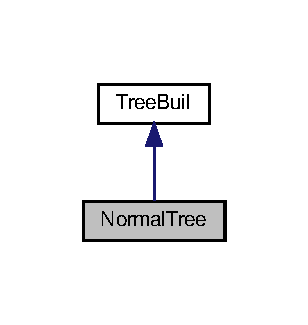
\includegraphics[width=148pt]{classNormalTree__inherit__graph}
\end{center}
\end{figure}


Diagrama de colaboración para Normal\+Tree\+:
\nopagebreak
\begin{figure}[H]
\begin{center}
\leavevmode
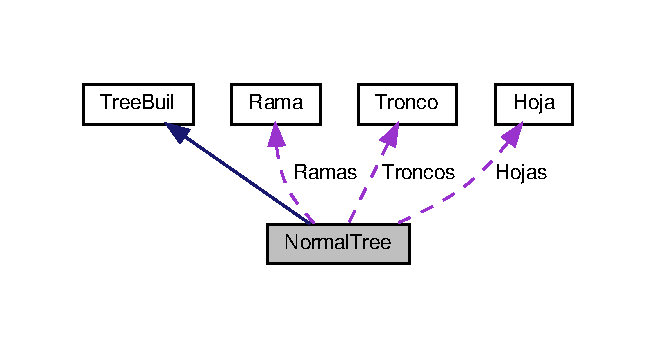
\includegraphics[width=315pt]{classNormalTree__coll__graph}
\end{center}
\end{figure}
\subsection*{Métodos públicos}
\begin{DoxyCompactItemize}
\item 
void \hyperlink{classNormalTree_a5b04a8afd8b44a3e2f82479da865f380}{set\+Tronco} (int size)
\item 
void \hyperlink{classNormalTree_a45a0b24a56264362ff1ab0ffa7843f2b}{set\+Hojas} (int size)
\item 
void \hyperlink{classNormalTree_aecf407fc3390d3011effea2f8dea464b}{set\+Ramas} (int size)
\item 
\hyperlink{classTronco}{Tronco} $\ast$ \hyperlink{classNormalTree_a95dcc1035a23a0142ace79e5f994e85a}{get\+Tronco} ()
\item 
\hyperlink{classHoja}{Hoja} $\ast$ \hyperlink{classNormalTree_af856515defde72c7d3350902bfe1cc3e}{get\+Hojas} ()
\item 
\hyperlink{classRama}{Rama} $\ast$ \hyperlink{classNormalTree_ad96708fd66844690669bd9d733b41063}{get\+Ramas} ()
\end{DoxyCompactItemize}
\subsection*{Atributos públicos}
\begin{DoxyCompactItemize}
\item 
\mbox{\Hypertarget{classNormalTree_a13483e7c3441eeaedb7fd6d5c6737f3b}\label{classNormalTree_a13483e7c3441eeaedb7fd6d5c6737f3b}} 
\hyperlink{classTronco}{Tronco} $\ast$ {\bfseries Troncos}
\item 
\mbox{\Hypertarget{classNormalTree_aeadff2f44c2e1a2449a92697149aefc1}\label{classNormalTree_aeadff2f44c2e1a2449a92697149aefc1}} 
\hyperlink{classHoja}{Hoja} $\ast$ {\bfseries Hojas}
\item 
\mbox{\Hypertarget{classNormalTree_a9247184649c047af5f905459539e3c61}\label{classNormalTree_a9247184649c047af5f905459539e3c61}} 
\hyperlink{classRama}{Rama} $\ast$ {\bfseries Ramas}
\end{DoxyCompactItemize}


\subsection{Descripción detallada}
La clase \hyperlink{classNormalTree}{Normal\+Tree} contiene las funciones get\+Tronco, get\+Hojas, get\+Ramas; asi como loset sets de estas para obtener y generar las caracteristicas del arbol  Las funciones apuntan a las clases de las partes del arbol, asi como tambien son void. 

\subsection{Documentación de las funciones miembro}
\mbox{\Hypertarget{classNormalTree_af856515defde72c7d3350902bfe1cc3e}\label{classNormalTree_af856515defde72c7d3350902bfe1cc3e}} 
\index{Normal\+Tree@{Normal\+Tree}!get\+Hojas@{get\+Hojas}}
\index{get\+Hojas@{get\+Hojas}!Normal\+Tree@{Normal\+Tree}}
\subsubsection{\texorpdfstring{get\+Hojas()}{getHojas()}}
{\footnotesize\ttfamily \hyperlink{classHoja}{Hoja} $\ast$ Normal\+Tree\+::get\+Hojas (\begin{DoxyParamCaption}{ }\end{DoxyParamCaption})\hspace{0.3cm}{\ttfamily [virtual]}}

La funcion get\+Hojas es un puntero a \hyperlink{classTronco}{Tronco}, nos permite obtener las caracteristicas de este. 

Implementa \hyperlink{classTreeBuil_a76ddaf2d79386ffabe5bf17e0c6d887e}{Tree\+Buil}.

\mbox{\Hypertarget{classNormalTree_ad96708fd66844690669bd9d733b41063}\label{classNormalTree_ad96708fd66844690669bd9d733b41063}} 
\index{Normal\+Tree@{Normal\+Tree}!get\+Ramas@{get\+Ramas}}
\index{get\+Ramas@{get\+Ramas}!Normal\+Tree@{Normal\+Tree}}
\subsubsection{\texorpdfstring{get\+Ramas()}{getRamas()}}
{\footnotesize\ttfamily \hyperlink{classRama}{Rama} $\ast$ Normal\+Tree\+::get\+Ramas (\begin{DoxyParamCaption}{ }\end{DoxyParamCaption})\hspace{0.3cm}{\ttfamily [virtual]}}

La funcion get\+Ramas es un puntero a \hyperlink{classTronco}{Tronco}, nos permite obtener las caracteristicas de este. 

Implementa \hyperlink{classTreeBuil_ad8c90d4466a151a8082eeae13400e6cc}{Tree\+Buil}.

\mbox{\Hypertarget{classNormalTree_a95dcc1035a23a0142ace79e5f994e85a}\label{classNormalTree_a95dcc1035a23a0142ace79e5f994e85a}} 
\index{Normal\+Tree@{Normal\+Tree}!get\+Tronco@{get\+Tronco}}
\index{get\+Tronco@{get\+Tronco}!Normal\+Tree@{Normal\+Tree}}
\subsubsection{\texorpdfstring{get\+Tronco()}{getTronco()}}
{\footnotesize\ttfamily \hyperlink{classTronco}{Tronco} $\ast$ Normal\+Tree\+::get\+Tronco (\begin{DoxyParamCaption}{ }\end{DoxyParamCaption})\hspace{0.3cm}{\ttfamily [virtual]}}

La funcion get\+Tronco es un puntero a \hyperlink{classTronco}{Tronco}, nos permite obtener las caracteristicas de este. 

Implementa \hyperlink{classTreeBuil_a083d65b3e44e233b9a2a9305bcdabb8c}{Tree\+Buil}.

\mbox{\Hypertarget{classNormalTree_a45a0b24a56264362ff1ab0ffa7843f2b}\label{classNormalTree_a45a0b24a56264362ff1ab0ffa7843f2b}} 
\index{Normal\+Tree@{Normal\+Tree}!set\+Hojas@{set\+Hojas}}
\index{set\+Hojas@{set\+Hojas}!Normal\+Tree@{Normal\+Tree}}
\subsubsection{\texorpdfstring{set\+Hojas()}{setHojas()}}
{\footnotesize\ttfamily void Normal\+Tree\+::set\+Hojas (\begin{DoxyParamCaption}\item[{int}]{size }\end{DoxyParamCaption})}

La funcion set\+Hojas recibe el tamano. 
\begin{DoxyParams}{Parámetros}
{\em size,nos} & permite definir el tamano pedido. \\
\hline
\end{DoxyParams}
\mbox{\Hypertarget{classNormalTree_aecf407fc3390d3011effea2f8dea464b}\label{classNormalTree_aecf407fc3390d3011effea2f8dea464b}} 
\index{Normal\+Tree@{Normal\+Tree}!set\+Ramas@{set\+Ramas}}
\index{set\+Ramas@{set\+Ramas}!Normal\+Tree@{Normal\+Tree}}
\subsubsection{\texorpdfstring{set\+Ramas()}{setRamas()}}
{\footnotesize\ttfamily void Normal\+Tree\+::set\+Ramas (\begin{DoxyParamCaption}\item[{int}]{size }\end{DoxyParamCaption})}

La funcion set\+Ramas recibe el tamano. 
\begin{DoxyParams}{Parámetros}
{\em size,nos} & permite definir el tamano pedido. \\
\hline
\end{DoxyParams}
\mbox{\Hypertarget{classNormalTree_a5b04a8afd8b44a3e2f82479da865f380}\label{classNormalTree_a5b04a8afd8b44a3e2f82479da865f380}} 
\index{Normal\+Tree@{Normal\+Tree}!set\+Tronco@{set\+Tronco}}
\index{set\+Tronco@{set\+Tronco}!Normal\+Tree@{Normal\+Tree}}
\subsubsection{\texorpdfstring{set\+Tronco()}{setTronco()}}
{\footnotesize\ttfamily void Normal\+Tree\+::set\+Tronco (\begin{DoxyParamCaption}\item[{int}]{size }\end{DoxyParamCaption})}

La funcion set\+Tronco recibe el tamano. 
\begin{DoxyParams}{Parámetros}
{\em size,nos} & permite definir el tamano pedido. \\
\hline
\end{DoxyParams}


La documentación para esta clase fue generada a partir de los siguientes ficheros\+:\begin{DoxyCompactItemize}
\item 
\hyperlink{ArbolBuilder_8h}{Arbol\+Builder.\+h}\item 
Arbol\+Builder.\+cpp\end{DoxyCompactItemize}

\hypertarget{classParticle}{}\section{Referencia de la Clase Particle}
\label{classParticle}\index{Particle@{Particle}}


La clase \hyperlink{classParticle}{Particle} contiene las funciones display para poder visualizarlo, set cant y gv  Se instancia el dato miembro para cantidad y gv para los pixels que recorre por iteracion.  




{\ttfamily \#include $<$Parti\+Flyweight.\+h$>$}

\subsection*{Métodos públicos}
\begin{DoxyCompactItemize}
\item 
\mbox{\Hypertarget{classParticle_ab565c9d9aa94223ba60335215701e88f}\label{classParticle_ab565c9d9aa94223ba60335215701e88f}} 
{\bfseries Particle} (int \+\_\+tam)
\item 
void \hyperlink{classParticle_abd939556d3a09985d90db3dd13809c5c}{set\+Tam} (int tam)
\item 
void \hyperlink{classParticle_a8a6aaeb2562d8540f42e5f63215bd207}{set\+XY} (int \+\_\+x, int \+\_\+y)
\item 
void \hyperlink{classParticle_ab9e7c76c8d36b1bf5082c6284ac515f7}{display} (\hyperlink{classTurtle}{Turtle} T)
\end{DoxyCompactItemize}


\subsection{Descripción detallada}
La clase \hyperlink{classParticle}{Particle} contiene las funciones display para poder visualizarlo, set cant y gv  Se instancia el dato miembro para cantidad y gv para los pixels que recorre por iteracion. 

\subsection{Documentación de las funciones miembro}
\mbox{\Hypertarget{classParticle_ab9e7c76c8d36b1bf5082c6284ac515f7}\label{classParticle_ab9e7c76c8d36b1bf5082c6284ac515f7}} 
\index{Particle@{Particle}!display@{display}}
\index{display@{display}!Particle@{Particle}}
\subsubsection{\texorpdfstring{display()}{display()}}
{\footnotesize\ttfamily void Particle\+::display (\begin{DoxyParamCaption}\item[{\hyperlink{classTurtle}{Turtle}}]{T }\end{DoxyParamCaption})}

La funcion display recibe la tortuga. 
\begin{DoxyParams}{Parámetros}
{\em T,recibe} & la tortuga para poder dibujar. \\
\hline
\end{DoxyParams}
\mbox{\Hypertarget{classParticle_abd939556d3a09985d90db3dd13809c5c}\label{classParticle_abd939556d3a09985d90db3dd13809c5c}} 
\index{Particle@{Particle}!set\+Tam@{set\+Tam}}
\index{set\+Tam@{set\+Tam}!Particle@{Particle}}
\subsubsection{\texorpdfstring{set\+Tam()}{setTam()}}
{\footnotesize\ttfamily void Particle\+::set\+Tam (\begin{DoxyParamCaption}\item[{int}]{tam }\end{DoxyParamCaption})\hspace{0.3cm}{\ttfamily [inline]}}

La funcion set\+Tam da el tamano. 
\begin{DoxyParams}{Parámetros}
{\em tam,da} & el tamano de la particula por crear. \\
\hline
\end{DoxyParams}
\mbox{\Hypertarget{classParticle_a8a6aaeb2562d8540f42e5f63215bd207}\label{classParticle_a8a6aaeb2562d8540f42e5f63215bd207}} 
\index{Particle@{Particle}!set\+XY@{set\+XY}}
\index{set\+XY@{set\+XY}!Particle@{Particle}}
\subsubsection{\texorpdfstring{set\+X\+Y()}{setXY()}}
{\footnotesize\ttfamily void Particle\+::set\+XY (\begin{DoxyParamCaption}\item[{int}]{\+\_\+x,  }\item[{int}]{\+\_\+y }\end{DoxyParamCaption})}

La funcion set\+XY da a conocer las coordenadas para que se realica ahi la creacion del objeto. 
\begin{DoxyParams}{Parámetros}
{\em \+\_\+x,\+\_\+y} & genera las coordenadas x, y del objeto. \\
\hline
\end{DoxyParams}


La documentación para esta clase fue generada a partir de los siguientes ficheros\+:\begin{DoxyCompactItemize}
\item 
\hyperlink{PartiFlyweight_8h}{Parti\+Flyweight.\+h}\item 
Parti\+Flyweight.\+cpp\end{DoxyCompactItemize}

\hypertarget{classPrim}{}\section{Referencia de la Clase Prim}
\label{classPrim}\index{Prim@{Prim}}


La clase \hyperlink{classPrim}{Prim} es la clase \hyperlink{classAbstractFact}{Abstract\+Fact} concreta  Se instancian punteros a cada uno de nuestros objetos.  




{\ttfamily \#include $<$Abstract.\+h$>$}



Diagrama de herencias de Prim\nopagebreak
\begin{figure}[H]
\begin{center}
\leavevmode
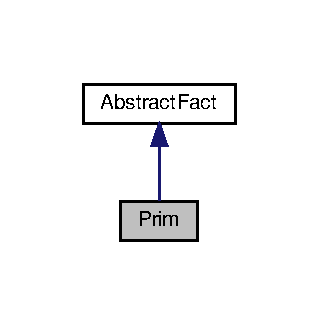
\includegraphics[width=153pt]{classPrim__inherit__graph}
\end{center}
\end{figure}


Diagrama de colaboración para Prim\+:\nopagebreak
\begin{figure}[H]
\begin{center}
\leavevmode
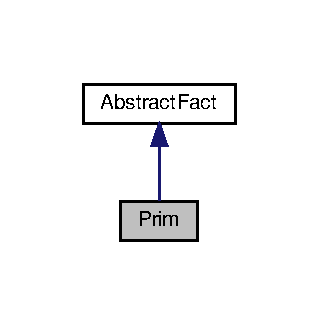
\includegraphics[width=153pt]{classPrim__coll__graph}
\end{center}
\end{figure}
\subsection*{Métodos públicos}
\begin{DoxyCompactItemize}
\item 
\hyperlink{classTree}{Tree} $\ast$ \hyperlink{classPrim_aeccbb4f2821f8bc508647e2f6dd95370}{get\+Tree} ()
\item 
\hyperlink{classFlower}{Flower} $\ast$ \hyperlink{classPrim_a92e3d118382a67173d008d5d82e4798c}{get\+Flor} ()
\item 
\hyperlink{classSnow}{Snow} $\ast$ \hyperlink{classPrim_ae2c1e853547a33662bd00baff26d67f8}{get\+Parti} ()
\end{DoxyCompactItemize}


\subsection{Descripción detallada}
La clase \hyperlink{classPrim}{Prim} es la clase \hyperlink{classAbstractFact}{Abstract\+Fact} concreta  Se instancian punteros a cada uno de nuestros objetos. 

\subsection{Documentación de las funciones miembro}
\mbox{\Hypertarget{classPrim_a92e3d118382a67173d008d5d82e4798c}\label{classPrim_a92e3d118382a67173d008d5d82e4798c}} 
\index{Prim@{Prim}!get\+Flor@{get\+Flor}}
\index{get\+Flor@{get\+Flor}!Prim@{Prim}}
\subsubsection{\texorpdfstring{get\+Flor()}{getFlor()}}
{\footnotesize\ttfamily \hyperlink{classFlower}{Flower} $\ast$ Prim\+::get\+Flor (\begin{DoxyParamCaption}{ }\end{DoxyParamCaption})\hspace{0.3cm}{\ttfamily [virtual]}}

Funcion para poder obetener nuestra flor tipo \hyperlink{classPrim}{Prim}. 

Implementa \hyperlink{classAbstractFact_a9ee9f34bc189886b24e325ff2412a1d9}{Abstract\+Fact}.

\mbox{\Hypertarget{classPrim_ae2c1e853547a33662bd00baff26d67f8}\label{classPrim_ae2c1e853547a33662bd00baff26d67f8}} 
\index{Prim@{Prim}!get\+Parti@{get\+Parti}}
\index{get\+Parti@{get\+Parti}!Prim@{Prim}}
\subsubsection{\texorpdfstring{get\+Parti()}{getParti()}}
{\footnotesize\ttfamily \hyperlink{classSnow}{Snow} $\ast$ Prim\+::get\+Parti (\begin{DoxyParamCaption}{ }\end{DoxyParamCaption})\hspace{0.3cm}{\ttfamily [virtual]}}

Funcion para poder obetener nuestra nieve tipo \hyperlink{classPrim}{Prim}. 

Implementa \hyperlink{classAbstractFact_a7b642a7fe5615f7103dd7d1ab4c801d9}{Abstract\+Fact}.

\mbox{\Hypertarget{classPrim_aeccbb4f2821f8bc508647e2f6dd95370}\label{classPrim_aeccbb4f2821f8bc508647e2f6dd95370}} 
\index{Prim@{Prim}!get\+Tree@{get\+Tree}}
\index{get\+Tree@{get\+Tree}!Prim@{Prim}}
\subsubsection{\texorpdfstring{get\+Tree()}{getTree()}}
{\footnotesize\ttfamily \hyperlink{classTree}{Tree} $\ast$ Prim\+::get\+Tree (\begin{DoxyParamCaption}{ }\end{DoxyParamCaption})\hspace{0.3cm}{\ttfamily [virtual]}}

Funcion para poder obetener nuestro arbol tipo \hyperlink{classPrim}{Prim}. 

Implementa \hyperlink{classAbstractFact_a37e763c0a454db79c61f229d33b72c73}{Abstract\+Fact}.



La documentación para esta clase fue generada a partir de los siguientes ficheros\+:\begin{DoxyCompactItemize}
\item 
\hyperlink{Abstract_8h}{Abstract.\+h}\item 
Abstract.\+cpp\end{DoxyCompactItemize}

\hypertarget{classRama}{}\section{Referencia de la Clase Rama}
\label{classRama}\index{Rama@{Rama}}


La clase \hyperlink{classRama}{Rama} contiene la funcion drawn para poder visualizarlo  Se instancia el dato miembro.  




{\ttfamily \#include $<$Arbol\+Builder.\+h$>$}

\subsection*{Métodos públicos}
\begin{DoxyCompactItemize}
\item 
void \hyperlink{classRama_af3c32428c96a45d6ef53b1828a66073d}{drawn} (\hyperlink{classTurtle}{Turtle} T, int x, int y)
\end{DoxyCompactItemize}
\subsection*{Atributos públicos}
\begin{DoxyCompactItemize}
\item 
\mbox{\Hypertarget{classRama_a679c0891200cfad9130a13c7d44e3fa5}\label{classRama_a679c0891200cfad9130a13c7d44e3fa5}} 
int {\bfseries size}
\end{DoxyCompactItemize}


\subsection{Descripción detallada}
La clase \hyperlink{classRama}{Rama} contiene la funcion drawn para poder visualizarlo  Se instancia el dato miembro. 

\subsection{Documentación de las funciones miembro}
\mbox{\Hypertarget{classRama_af3c32428c96a45d6ef53b1828a66073d}\label{classRama_af3c32428c96a45d6ef53b1828a66073d}} 
\index{Rama@{Rama}!drawn@{drawn}}
\index{drawn@{drawn}!Rama@{Rama}}
\subsubsection{\texorpdfstring{drawn()}{drawn()}}
{\footnotesize\ttfamily void Rama\+::drawn (\begin{DoxyParamCaption}\item[{\hyperlink{classTurtle}{Turtle}}]{T,  }\item[{int}]{x,  }\item[{int}]{y }\end{DoxyParamCaption})}

La funcion drawn recibe la tortuga y el tamano. 
\begin{DoxyParams}{Parámetros}
{\em T,nos} & permite hacer uso de la tortuga y x, y coordinan el tamano de la rama. \\
\hline
\end{DoxyParams}


La documentación para esta clase fue generada a partir de los siguientes ficheros\+:\begin{DoxyCompactItemize}
\item 
\hyperlink{ArbolBuilder_8h}{Arbol\+Builder.\+h}\item 
Arbol\+Builder.\+cpp\end{DoxyCompactItemize}

\hypertarget{classSeco}{}\section{Referencia de la Clase Seco}
\label{classSeco}\index{Seco@{Seco}}


La clase \hyperlink{classSeco}{Seco} es la clase \hyperlink{classAbstractFact}{Abstract\+Fact} concreta  Se instancian punteros a cada uno de nuestros objetos pero esta vez de otro tipo.  




{\ttfamily \#include $<$Abstract.\+h$>$}



Diagrama de herencias de Seco\nopagebreak
\begin{figure}[H]
\begin{center}
\leavevmode
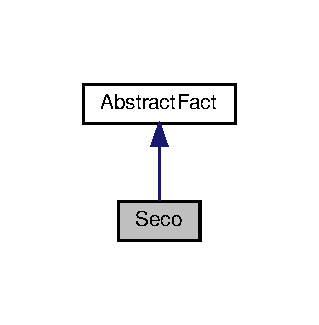
\includegraphics[width=153pt]{classSeco__inherit__graph}
\end{center}
\end{figure}


Diagrama de colaboración para Seco\+:\nopagebreak
\begin{figure}[H]
\begin{center}
\leavevmode
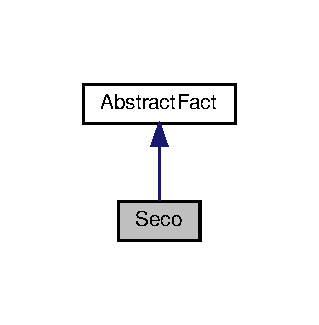
\includegraphics[width=153pt]{classSeco__coll__graph}
\end{center}
\end{figure}
\subsection*{Métodos públicos}
\begin{DoxyCompactItemize}
\item 
\hyperlink{classTree}{Tree} $\ast$ \hyperlink{classSeco_ae4a078cccba29b3d89dcb62b6eeaa269}{get\+Tree} ()
\item 
\hyperlink{classFlower}{Flower} $\ast$ \hyperlink{classSeco_a91092401b16231a926255323e89c6412}{get\+Flor} ()
\item 
\hyperlink{classSnow}{Snow} $\ast$ \hyperlink{classSeco_acd61763141ecdb895062cdde7defa800}{get\+Parti} ()
\end{DoxyCompactItemize}


\subsection{Descripción detallada}
La clase \hyperlink{classSeco}{Seco} es la clase \hyperlink{classAbstractFact}{Abstract\+Fact} concreta  Se instancian punteros a cada uno de nuestros objetos pero esta vez de otro tipo. 

\subsection{Documentación de las funciones miembro}
\mbox{\Hypertarget{classSeco_a91092401b16231a926255323e89c6412}\label{classSeco_a91092401b16231a926255323e89c6412}} 
\index{Seco@{Seco}!get\+Flor@{get\+Flor}}
\index{get\+Flor@{get\+Flor}!Seco@{Seco}}
\subsubsection{\texorpdfstring{get\+Flor()}{getFlor()}}
{\footnotesize\ttfamily \hyperlink{classFlower}{Flower} $\ast$ Seco\+::get\+Flor (\begin{DoxyParamCaption}{ }\end{DoxyParamCaption})\hspace{0.3cm}{\ttfamily [virtual]}}

Funcion para poder obetener nuestra flor tipo \hyperlink{classSeco}{Seco}. 

Implementa \hyperlink{classAbstractFact_a9ee9f34bc189886b24e325ff2412a1d9}{Abstract\+Fact}.

\mbox{\Hypertarget{classSeco_acd61763141ecdb895062cdde7defa800}\label{classSeco_acd61763141ecdb895062cdde7defa800}} 
\index{Seco@{Seco}!get\+Parti@{get\+Parti}}
\index{get\+Parti@{get\+Parti}!Seco@{Seco}}
\subsubsection{\texorpdfstring{get\+Parti()}{getParti()}}
{\footnotesize\ttfamily \hyperlink{classSnow}{Snow} $\ast$ Seco\+::get\+Parti (\begin{DoxyParamCaption}{ }\end{DoxyParamCaption})\hspace{0.3cm}{\ttfamily [virtual]}}

Funcion para poder obetener nuestra nieve tipo \hyperlink{classSeco}{Seco}. 

Implementa \hyperlink{classAbstractFact_a7b642a7fe5615f7103dd7d1ab4c801d9}{Abstract\+Fact}.

\mbox{\Hypertarget{classSeco_ae4a078cccba29b3d89dcb62b6eeaa269}\label{classSeco_ae4a078cccba29b3d89dcb62b6eeaa269}} 
\index{Seco@{Seco}!get\+Tree@{get\+Tree}}
\index{get\+Tree@{get\+Tree}!Seco@{Seco}}
\subsubsection{\texorpdfstring{get\+Tree()}{getTree()}}
{\footnotesize\ttfamily \hyperlink{classTree}{Tree} $\ast$ Seco\+::get\+Tree (\begin{DoxyParamCaption}{ }\end{DoxyParamCaption})\hspace{0.3cm}{\ttfamily [virtual]}}

Funcion para poder obetener nuestro arbol tipo \hyperlink{classSeco}{Seco}. 

Implementa \hyperlink{classAbstractFact_a37e763c0a454db79c61f229d33b72c73}{Abstract\+Fact}.



La documentación para esta clase fue generada a partir de los siguientes ficheros\+:\begin{DoxyCompactItemize}
\item 
\hyperlink{Abstract_8h}{Abstract.\+h}\item 
Abstract.\+cpp\end{DoxyCompactItemize}

\hypertarget{classSnow}{}\section{Referencia de la Clase Snow}
\label{classSnow}\index{Snow@{Snow}}


La clase \hyperlink{classSnow}{Snow} contiene las funciones display para poder visualizarlo, set cant y gv  Se instancia el dato miembro para cantidad, gv para los pixels que recorre por iteracion, un vector de particulas para guardar las que son pedidas por el usuario.  




{\ttfamily \#include $<$Parti\+Flyweight.\+h$>$}

\subsection*{Métodos públicos}
\begin{DoxyCompactItemize}
\item 
\hyperlink{classSnow_afe2f36ed0e41531355273259e6ad339f}{Snow} (int \+\_\+tam=3)
\item 
\hyperlink{classSnow_a8bf279bbf1ddd5b180692797996ce7b5}{$\sim$\+Snow} ()
\item 
void \hyperlink{classSnow_a624263662e99a3d80022a86be73588f2}{display} (\hyperlink{classTurtle}{Turtle} T)
\item 
void \hyperlink{classSnow_a3cabcbee15d87f551d90be472f1865c4}{setC} (int \+\_\+c)
\item 
void \hyperlink{classSnow_a7b77940da35738cd518c5c66d04350cf}{set\+Gv} (int \+\_\+gv)
\item 
void \hyperlink{classSnow_a441e42b0e5cee4d21220b243e08b344d}{insert} (int tam)
\end{DoxyCompactItemize}


\subsection{Descripción detallada}
La clase \hyperlink{classSnow}{Snow} contiene las funciones display para poder visualizarlo, set cant y gv  Se instancia el dato miembro para cantidad, gv para los pixels que recorre por iteracion, un vector de particulas para guardar las que son pedidas por el usuario. 

\subsection{Documentación del constructor y destructor}
\mbox{\Hypertarget{classSnow_afe2f36ed0e41531355273259e6ad339f}\label{classSnow_afe2f36ed0e41531355273259e6ad339f}} 
\index{Snow@{Snow}!Snow@{Snow}}
\index{Snow@{Snow}!Snow@{Snow}}
\subsubsection{\texorpdfstring{Snow()}{Snow()}}
{\footnotesize\ttfamily Snow\+::\+Snow (\begin{DoxyParamCaption}\item[{int}]{\+\_\+tam = {\ttfamily 3} }\end{DoxyParamCaption})}

Constructor. 
\begin{DoxyParams}{Parámetros}
{\em \+\_\+tam} & es el tamaño de cada copo de nieve. \\
\hline
\end{DoxyParams}
\mbox{\Hypertarget{classSnow_a8bf279bbf1ddd5b180692797996ce7b5}\label{classSnow_a8bf279bbf1ddd5b180692797996ce7b5}} 
\index{Snow@{Snow}!````~Snow@{$\sim$\+Snow}}
\index{````~Snow@{$\sim$\+Snow}!Snow@{Snow}}
\subsubsection{\texorpdfstring{$\sim$\+Snow()}{~Snow()}}
{\footnotesize\ttfamily Snow\+::$\sim$\+Snow (\begin{DoxyParamCaption}{ }\end{DoxyParamCaption})}

Destructor. 

\subsection{Documentación de las funciones miembro}
\mbox{\Hypertarget{classSnow_a624263662e99a3d80022a86be73588f2}\label{classSnow_a624263662e99a3d80022a86be73588f2}} 
\index{Snow@{Snow}!display@{display}}
\index{display@{display}!Snow@{Snow}}
\subsubsection{\texorpdfstring{display()}{display()}}
{\footnotesize\ttfamily void Snow\+::display (\begin{DoxyParamCaption}\item[{\hyperlink{classTurtle}{Turtle}}]{T }\end{DoxyParamCaption})}

La funcion display muestra el objeto. 
\begin{DoxyParams}{Parámetros}
{\em T} & recibe la tortuga para que sea utlizada en la funcion. \\
\hline
\end{DoxyParams}
\mbox{\Hypertarget{classSnow_a441e42b0e5cee4d21220b243e08b344d}\label{classSnow_a441e42b0e5cee4d21220b243e08b344d}} 
\index{Snow@{Snow}!insert@{insert}}
\index{insert@{insert}!Snow@{Snow}}
\subsubsection{\texorpdfstring{insert()}{insert()}}
{\footnotesize\ttfamily void Snow\+::insert (\begin{DoxyParamCaption}\item[{int}]{tam }\end{DoxyParamCaption})}

La funcion insert agrega particulas a nuestro vector. 
\begin{DoxyParams}{Parámetros}
{\em tam,tamano} & de las particulas que se van a generar \\
\hline
\end{DoxyParams}
\mbox{\Hypertarget{classSnow_a3cabcbee15d87f551d90be472f1865c4}\label{classSnow_a3cabcbee15d87f551d90be472f1865c4}} 
\index{Snow@{Snow}!setC@{setC}}
\index{setC@{setC}!Snow@{Snow}}
\subsubsection{\texorpdfstring{set\+C()}{setC()}}
{\footnotesize\ttfamily void Snow\+::setC (\begin{DoxyParamCaption}\item[{int}]{\+\_\+c }\end{DoxyParamCaption})}

La funcion setC define la cantidad de copos de nieve que habra en el plano. 
\begin{DoxyParams}{Parámetros}
{\em \+\_\+cant} & la cantidad de copos de nieve. \\
\hline
\end{DoxyParams}
\mbox{\Hypertarget{classSnow_a7b77940da35738cd518c5c66d04350cf}\label{classSnow_a7b77940da35738cd518c5c66d04350cf}} 
\index{Snow@{Snow}!set\+Gv@{set\+Gv}}
\index{set\+Gv@{set\+Gv}!Snow@{Snow}}
\subsubsection{\texorpdfstring{set\+Gv()}{setGv()}}
{\footnotesize\ttfamily void Snow\+::set\+Gv (\begin{DoxyParamCaption}\item[{int}]{\+\_\+gv }\end{DoxyParamCaption})}

La funcion set\+Gv define la cantidad de pixeles en la que de nieve que habra en el plano. 
\begin{DoxyParams}{Parámetros}
{\em \+\_\+grave} & los pixeles de gravedad que tendra. \\
\hline
\end{DoxyParams}


La documentación para esta clase fue generada a partir de los siguientes ficheros\+:\begin{DoxyCompactItemize}
\item 
\hyperlink{PartiFlyweight_8h}{Parti\+Flyweight.\+h}\item 
Parti\+Flyweight.\+cpp\end{DoxyCompactItemize}

\hypertarget{classSnowFly}{}\section{Referencia de la Clase Snow\+Fly}
\label{classSnowFly}\index{Snow\+Fly@{Snow\+Fly}}


La clase \hyperlink{classSnowFly}{Snow\+Fly} contiene las funciones set\+Tam y get\+Tam para poder darle tamano a nuesta nieve  Se instancia el dato miembro tam.  




{\ttfamily \#include $<$Parti\+Flyweight.\+h$>$}



Diagrama de colaboración para Snow\+Fly\+:\nopagebreak
\begin{figure}[H]
\begin{center}
\leavevmode
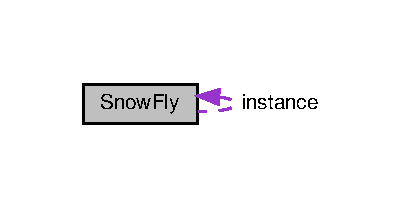
\includegraphics[width=193pt]{classSnowFly__coll__graph}
\end{center}
\end{figure}
\subsection*{Métodos públicos}
\begin{DoxyCompactItemize}
\item 
void \hyperlink{classSnowFly_a1068f2ce770daa2932732ec6c94715a9}{set\+Tam} (int \+\_\+tam)
\item 
int \hyperlink{classSnowFly_a6677ebdc7b0cb9bb7ea1b90292b18ef2}{get\+Tam} ()
\end{DoxyCompactItemize}
\subsection*{Métodos públicos estáticos}
\begin{DoxyCompactItemize}
\item 
\mbox{\Hypertarget{classSnowFly_a2a1b39f6b9f85311222e82e68d131650}\label{classSnowFly_a2a1b39f6b9f85311222e82e68d131650}} 
static \hyperlink{classSnowFly}{Snow\+Fly} $\ast$ {\bfseries get\+Instance} ()
\end{DoxyCompactItemize}
\subsection*{Atributos públicos estáticos}
\begin{DoxyCompactItemize}
\item 
\mbox{\Hypertarget{classSnowFly_a7d6143f2d7e5fb5650afca3f6436f208}\label{classSnowFly_a7d6143f2d7e5fb5650afca3f6436f208}} 
static \hyperlink{classSnowFly}{Snow\+Fly} $\ast$ {\bfseries instance} = 0
\end{DoxyCompactItemize}


\subsection{Descripción detallada}
La clase \hyperlink{classSnowFly}{Snow\+Fly} contiene las funciones set\+Tam y get\+Tam para poder darle tamano a nuesta nieve  Se instancia el dato miembro tam. 

\subsection{Documentación de las funciones miembro}
\mbox{\Hypertarget{classSnowFly_a6677ebdc7b0cb9bb7ea1b90292b18ef2}\label{classSnowFly_a6677ebdc7b0cb9bb7ea1b90292b18ef2}} 
\index{Snow\+Fly@{Snow\+Fly}!get\+Tam@{get\+Tam}}
\index{get\+Tam@{get\+Tam}!Snow\+Fly@{Snow\+Fly}}
\subsubsection{\texorpdfstring{get\+Tam()}{getTam()}}
{\footnotesize\ttfamily int Snow\+Fly\+::get\+Tam (\begin{DoxyParamCaption}{ }\end{DoxyParamCaption})}

La funcion get\+Tam obtiene el tamano. \mbox{\Hypertarget{classSnowFly_a1068f2ce770daa2932732ec6c94715a9}\label{classSnowFly_a1068f2ce770daa2932732ec6c94715a9}} 
\index{Snow\+Fly@{Snow\+Fly}!set\+Tam@{set\+Tam}}
\index{set\+Tam@{set\+Tam}!Snow\+Fly@{Snow\+Fly}}
\subsubsection{\texorpdfstring{set\+Tam()}{setTam()}}
{\footnotesize\ttfamily void Snow\+Fly\+::set\+Tam (\begin{DoxyParamCaption}\item[{int}]{\+\_\+tam }\end{DoxyParamCaption})}

La funcion set\+Tam da el tamano. 
\begin{DoxyParams}{Parámetros}
{\em \+\_\+tam} & recibe el tamano de los copos \\
\hline
\end{DoxyParams}


La documentación para esta clase fue generada a partir de los siguientes ficheros\+:\begin{DoxyCompactItemize}
\item 
\hyperlink{PartiFlyweight_8h}{Parti\+Flyweight.\+h}\item 
Parti\+Flyweight.\+cpp\end{DoxyCompactItemize}

\hypertarget{classTree}{}\section{Referencia de la Clase Tree}
\label{classTree}\index{Tree@{Tree}}


La clase \hyperlink{classTree}{Tree} contiene la funcion drawn para visualizar el arbol  Se instancia los datos miembros que son punteros a las partes del arbol.  




{\ttfamily \#include $<$Arbol\+Builder.\+h$>$}



Diagrama de colaboración para Tree\+:
\nopagebreak
\begin{figure}[H]
\begin{center}
\leavevmode
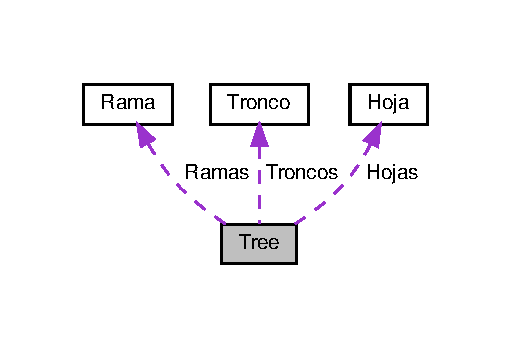
\includegraphics[width=245pt]{classTree__coll__graph}
\end{center}
\end{figure}
\subsection*{Métodos públicos}
\begin{DoxyCompactItemize}
\item 
void \hyperlink{classTree_aeb680a32bf1743d52cf63da53712dc7d}{drawn} (\hyperlink{classTurtle}{Turtle} T, int x, int y)
\end{DoxyCompactItemize}
\subsection*{Atributos públicos}
\begin{DoxyCompactItemize}
\item 
\mbox{\Hypertarget{classTree_a96e70d44324ad226b6a7fc1576ee7554}\label{classTree_a96e70d44324ad226b6a7fc1576ee7554}} 
\hyperlink{classTronco}{Tronco} $\ast$ {\bfseries Troncos}
\item 
\mbox{\Hypertarget{classTree_a8651c39bf1509dca86eb9fdd872581e0}\label{classTree_a8651c39bf1509dca86eb9fdd872581e0}} 
\hyperlink{classHoja}{Hoja} $\ast$ {\bfseries Hojas}
\item 
\mbox{\Hypertarget{classTree_a61e6de64e4f19bcf92f3c1cff9f17441}\label{classTree_a61e6de64e4f19bcf92f3c1cff9f17441}} 
\hyperlink{classRama}{Rama} $\ast$ {\bfseries Ramas}
\end{DoxyCompactItemize}


\subsection{Descripción detallada}
La clase \hyperlink{classTree}{Tree} contiene la funcion drawn para visualizar el arbol  Se instancia los datos miembros que son punteros a las partes del arbol. 

\subsection{Documentación de las funciones miembro}
\mbox{\Hypertarget{classTree_aeb680a32bf1743d52cf63da53712dc7d}\label{classTree_aeb680a32bf1743d52cf63da53712dc7d}} 
\index{Tree@{Tree}!drawn@{drawn}}
\index{drawn@{drawn}!Tree@{Tree}}
\subsubsection{\texorpdfstring{drawn()}{drawn()}}
{\footnotesize\ttfamily void Tree\+::drawn (\begin{DoxyParamCaption}\item[{\hyperlink{classTurtle}{Turtle}}]{T,  }\item[{int}]{x,  }\item[{int}]{y }\end{DoxyParamCaption})}

La funcion drawn recibe la tortuga y el tamano. 
\begin{DoxyParams}{Parámetros}
{\em T,nos} & permite hacer uso de la tortuga y x, y coordinan el tamano de cada objeto. \\
\hline
\end{DoxyParams}


La documentación para esta clase fue generada a partir de los siguientes ficheros\+:\begin{DoxyCompactItemize}
\item 
\hyperlink{ArbolBuilder_8h}{Arbol\+Builder.\+h}\item 
Arbol\+Builder.\+cpp\end{DoxyCompactItemize}

\hypertarget{classTreeBuil}{}\section{Referencia de la Clase Tree\+Buil}
\label{classTreeBuil}\index{Tree\+Buil@{Tree\+Buil}}


La interfaz \hyperlink{classTreeBuil}{Tree\+Buil} contiene las funciones get\+Tronco, get\+Hojas, get\+Ramas para obtener las caracteristicas del arbol  Las funciones son virtual-\/puras y apuntan a las clases de las partes del arbol.  




{\ttfamily \#include $<$Arbol\+Builder.\+h$>$}



Diagrama de herencias de Tree\+Buil\nopagebreak
\begin{figure}[H]
\begin{center}
\leavevmode
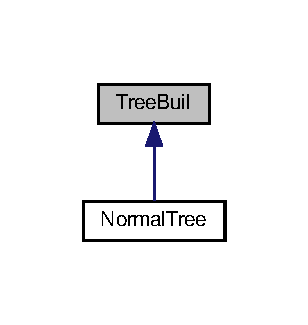
\includegraphics[width=148pt]{classTreeBuil__inherit__graph}
\end{center}
\end{figure}
\subsection*{Métodos públicos}
\begin{DoxyCompactItemize}
\item 
virtual \hyperlink{classTronco}{Tronco} $\ast$ \hyperlink{classTreeBuil_a083d65b3e44e233b9a2a9305bcdabb8c}{get\+Tronco} ()=0
\item 
virtual \hyperlink{classHoja}{Hoja} $\ast$ \hyperlink{classTreeBuil_a76ddaf2d79386ffabe5bf17e0c6d887e}{get\+Hojas} ()=0
\item 
virtual \hyperlink{classRama}{Rama} $\ast$ \hyperlink{classTreeBuil_ad8c90d4466a151a8082eeae13400e6cc}{get\+Ramas} ()=0
\end{DoxyCompactItemize}


\subsection{Descripción detallada}
La interfaz \hyperlink{classTreeBuil}{Tree\+Buil} contiene las funciones get\+Tronco, get\+Hojas, get\+Ramas para obtener las caracteristicas del arbol  Las funciones son virtual-\/puras y apuntan a las clases de las partes del arbol. 

\subsection{Documentación de las funciones miembro}
\mbox{\Hypertarget{classTreeBuil_a76ddaf2d79386ffabe5bf17e0c6d887e}\label{classTreeBuil_a76ddaf2d79386ffabe5bf17e0c6d887e}} 
\index{Tree\+Buil@{Tree\+Buil}!get\+Hojas@{get\+Hojas}}
\index{get\+Hojas@{get\+Hojas}!Tree\+Buil@{Tree\+Buil}}
\subsubsection{\texorpdfstring{get\+Hojas()}{getHojas()}}
{\footnotesize\ttfamily virtual \hyperlink{classHoja}{Hoja}$\ast$ Tree\+Buil\+::get\+Hojas (\begin{DoxyParamCaption}{ }\end{DoxyParamCaption})\hspace{0.3cm}{\ttfamily [pure virtual]}}

La funcion get\+Hojas es virtual pura para que pueda ser heredada, utilizada y sobrescrita por las demas clases. 

Implementado en \hyperlink{classNormalTree_af856515defde72c7d3350902bfe1cc3e}{Normal\+Tree}.

\mbox{\Hypertarget{classTreeBuil_ad8c90d4466a151a8082eeae13400e6cc}\label{classTreeBuil_ad8c90d4466a151a8082eeae13400e6cc}} 
\index{Tree\+Buil@{Tree\+Buil}!get\+Ramas@{get\+Ramas}}
\index{get\+Ramas@{get\+Ramas}!Tree\+Buil@{Tree\+Buil}}
\subsubsection{\texorpdfstring{get\+Ramas()}{getRamas()}}
{\footnotesize\ttfamily virtual \hyperlink{classRama}{Rama}$\ast$ Tree\+Buil\+::get\+Ramas (\begin{DoxyParamCaption}{ }\end{DoxyParamCaption})\hspace{0.3cm}{\ttfamily [pure virtual]}}

La funcion get\+Ramas es virtual pura para que pueda ser heredada, utilizada y sobrescrita por las demas clases. 

Implementado en \hyperlink{classNormalTree_ad96708fd66844690669bd9d733b41063}{Normal\+Tree}.

\mbox{\Hypertarget{classTreeBuil_a083d65b3e44e233b9a2a9305bcdabb8c}\label{classTreeBuil_a083d65b3e44e233b9a2a9305bcdabb8c}} 
\index{Tree\+Buil@{Tree\+Buil}!get\+Tronco@{get\+Tronco}}
\index{get\+Tronco@{get\+Tronco}!Tree\+Buil@{Tree\+Buil}}
\subsubsection{\texorpdfstring{get\+Tronco()}{getTronco()}}
{\footnotesize\ttfamily virtual \hyperlink{classTronco}{Tronco}$\ast$ Tree\+Buil\+::get\+Tronco (\begin{DoxyParamCaption}{ }\end{DoxyParamCaption})\hspace{0.3cm}{\ttfamily [pure virtual]}}

La funcion get\+Tronco es virtual pura para que pueda ser heredada, utilizada y sobrescrita por las demas clases. 

Implementado en \hyperlink{classNormalTree_a95dcc1035a23a0142ace79e5f994e85a}{Normal\+Tree}.



La documentación para esta clase fue generada a partir del siguiente fichero\+:\begin{DoxyCompactItemize}
\item 
\hyperlink{ArbolBuilder_8h}{Arbol\+Builder.\+h}\end{DoxyCompactItemize}

\hypertarget{classTronco}{}\section{Referencia de la Clase Tronco}
\label{classTronco}\index{Tronco@{Tronco}}


La clase \hyperlink{classTronco}{Tronco} contiene la funcion drawn para poder visualizarlo  Se instancia el dato miembro.  




{\ttfamily \#include $<$Arbol\+Builder.\+h$>$}

\subsection*{Métodos públicos}
\begin{DoxyCompactItemize}
\item 
void \hyperlink{classTronco_a0976269e055e451f0ca43059a46ea742}{drawn} (\hyperlink{classTurtle}{Turtle} T, int x, int y)
\end{DoxyCompactItemize}
\subsection*{Atributos públicos}
\begin{DoxyCompactItemize}
\item 
\mbox{\Hypertarget{classTronco_a34fac18044bfd5f785e795b0a6037c21}\label{classTronco_a34fac18044bfd5f785e795b0a6037c21}} 
int {\bfseries size}
\end{DoxyCompactItemize}


\subsection{Descripción detallada}
La clase \hyperlink{classTronco}{Tronco} contiene la funcion drawn para poder visualizarlo  Se instancia el dato miembro. 

\subsection{Documentación de las funciones miembro}
\mbox{\Hypertarget{classTronco_a0976269e055e451f0ca43059a46ea742}\label{classTronco_a0976269e055e451f0ca43059a46ea742}} 
\index{Tronco@{Tronco}!drawn@{drawn}}
\index{drawn@{drawn}!Tronco@{Tronco}}
\subsubsection{\texorpdfstring{drawn()}{drawn()}}
{\footnotesize\ttfamily void Tronco\+::drawn (\begin{DoxyParamCaption}\item[{\hyperlink{classTurtle}{Turtle}}]{T,  }\item[{int}]{x,  }\item[{int}]{y }\end{DoxyParamCaption})}

La funcion drawn recibe la tortuga y el tamano. 
\begin{DoxyParams}{Parámetros}
{\em T,nos} & permite hacer uso de la tortuga y x, y coordinan el tamano del tronco. \\
\hline
\end{DoxyParams}


La documentación para esta clase fue generada a partir de los siguientes ficheros\+:\begin{DoxyCompactItemize}
\item 
\hyperlink{ArbolBuilder_8h}{Arbol\+Builder.\+h}\item 
Arbol\+Builder.\+cpp\end{DoxyCompactItemize}

\hypertarget{classTurtle}{}\section{Referencia de la Clase Turtle}
\label{classTurtle}\index{Turtle@{Turtle}}


La clase tortuga contiene todos los metodos y funciones de \char`\"{}turtle\char`\"{} de Python  Una numeracion general sobre los metodos mas importantes de \char`\"{}turle\char`\"{}.  




{\ttfamily \#include $<$Turtle.\+h$>$}

\subsection*{Métodos públicos}
\begin{DoxyCompactItemize}
\item 
\hyperlink{classTurtle_a0a42aeefa221e7a0598e0af222214788}{Turtle} (int w1=500, int h1=500)
\item 
void \hyperlink{classTurtle_a8597b5fb6ad6abc2888a7246ffcf971c}{forward} (int di)
\item 
void \hyperlink{classTurtle_ad389432bb8cde6832c0fe1f76c891e94}{right} (double dg)
\item 
void \hyperlink{classTurtle_a8ba2af4d351e62de83ddfcc6bca51d9a}{left} (double dg)
\item 
void \hyperlink{classTurtle_a0cd2bf8afff89d89662f296dc781bb79}{backward} (int di)
\item 
void \hyperlink{classTurtle_ad4f1cfec231a2d91c529d20c2331168b}{set\+\_\+color} (int R, int G, int B)
\item 
void \hyperlink{classTurtle_a40367ef16bd84c7d382992b8e6d3a9fc}{penup} ()
\item 
void \hyperlink{classTurtle_aabe573f505a789dfe84fc2219ec0cb10}{pendow} ()
\item 
void \hyperlink{classTurtle_a486b5b199b51322309f969dd2c028fae}{move} (double x, double y)
\item 
void \hyperlink{classTurtle_ae62d0d6d90add2c86baa14ae01cdbe4a}{display} (int argc, char $\ast$$\ast$argv)
\item 
void \hyperlink{classTurtle_ad065d9fd92fa5eaee2b808f52c444838}{clear} ()
\end{DoxyCompactItemize}


\subsection{Descripción detallada}
La clase tortuga contiene todos los metodos y funciones de \char`\"{}turtle\char`\"{} de Python  Una numeracion general sobre los metodos mas importantes de \char`\"{}turle\char`\"{}. 

\subsection{Documentación del constructor y destructor}
\mbox{\Hypertarget{classTurtle_a0a42aeefa221e7a0598e0af222214788}\label{classTurtle_a0a42aeefa221e7a0598e0af222214788}} 
\index{Turtle@{Turtle}!Turtle@{Turtle}}
\index{Turtle@{Turtle}!Turtle@{Turtle}}
\subsubsection{\texorpdfstring{Turtle()}{Turtle()}}
{\footnotesize\ttfamily Turtle\+::\+Turtle (\begin{DoxyParamCaption}\item[{int}]{w1 = {\ttfamily 500},  }\item[{int}]{h1 = {\ttfamily 500} }\end{DoxyParamCaption})}

Constructor con tamano por defecto. 
\begin{DoxyParams}{Parámetros}
{\em w1,h2} & coordinan el tamano del plano. \\
\hline
\end{DoxyParams}


\subsection{Documentación de las funciones miembro}
\mbox{\Hypertarget{classTurtle_a0cd2bf8afff89d89662f296dc781bb79}\label{classTurtle_a0cd2bf8afff89d89662f296dc781bb79}} 
\index{Turtle@{Turtle}!backward@{backward}}
\index{backward@{backward}!Turtle@{Turtle}}
\subsubsection{\texorpdfstring{backward()}{backward()}}
{\footnotesize\ttfamily void Turtle\+::backward (\begin{DoxyParamCaption}\item[{int}]{di }\end{DoxyParamCaption})}

Funcion para retroceder. 
\begin{DoxyParams}{Parámetros}
{\em di,tamano} & de la linea recta por retroceder \\
\hline
\end{DoxyParams}
\mbox{\Hypertarget{classTurtle_ad065d9fd92fa5eaee2b808f52c444838}\label{classTurtle_ad065d9fd92fa5eaee2b808f52c444838}} 
\index{Turtle@{Turtle}!clear@{clear}}
\index{clear@{clear}!Turtle@{Turtle}}
\subsubsection{\texorpdfstring{clear()}{clear()}}
{\footnotesize\ttfamily void Turtle\+::clear (\begin{DoxyParamCaption}{ }\end{DoxyParamCaption})\hspace{0.3cm}{\ttfamily [inline]}}

limpiar ventana. \mbox{\Hypertarget{classTurtle_ae62d0d6d90add2c86baa14ae01cdbe4a}\label{classTurtle_ae62d0d6d90add2c86baa14ae01cdbe4a}} 
\index{Turtle@{Turtle}!display@{display}}
\index{display@{display}!Turtle@{Turtle}}
\subsubsection{\texorpdfstring{display()}{display()}}
{\footnotesize\ttfamily void Turtle\+::display (\begin{DoxyParamCaption}\item[{int}]{argc,  }\item[{char $\ast$$\ast$}]{argv }\end{DoxyParamCaption})}

mostrar ventana. 
\begin{DoxyParams}{Parámetros}
{\em argc,argv} & es necesario para la funcion glut\+Init. \\
\hline
\end{DoxyParams}
\mbox{\Hypertarget{classTurtle_a8597b5fb6ad6abc2888a7246ffcf971c}\label{classTurtle_a8597b5fb6ad6abc2888a7246ffcf971c}} 
\index{Turtle@{Turtle}!forward@{forward}}
\index{forward@{forward}!Turtle@{Turtle}}
\subsubsection{\texorpdfstring{forward()}{forward()}}
{\footnotesize\ttfamily void Turtle\+::forward (\begin{DoxyParamCaption}\item[{int}]{di }\end{DoxyParamCaption})}

Funcion para avanzar. 
\begin{DoxyParams}{Parámetros}
{\em di,tamano} & de la linea recta por avenzar \\
\hline
\end{DoxyParams}
\mbox{\Hypertarget{classTurtle_a8ba2af4d351e62de83ddfcc6bca51d9a}\label{classTurtle_a8ba2af4d351e62de83ddfcc6bca51d9a}} 
\index{Turtle@{Turtle}!left@{left}}
\index{left@{left}!Turtle@{Turtle}}
\subsubsection{\texorpdfstring{left()}{left()}}
{\footnotesize\ttfamily void Turtle\+::left (\begin{DoxyParamCaption}\item[{double}]{dg }\end{DoxyParamCaption})}

Gira a la izquierda los grados que recibe. 
\begin{DoxyParams}{Parámetros}
{\em dg,es} & la cantidad de grados que gira. \\
\hline
\end{DoxyParams}
\mbox{\Hypertarget{classTurtle_a486b5b199b51322309f969dd2c028fae}\label{classTurtle_a486b5b199b51322309f969dd2c028fae}} 
\index{Turtle@{Turtle}!move@{move}}
\index{move@{move}!Turtle@{Turtle}}
\subsubsection{\texorpdfstring{move()}{move()}}
{\footnotesize\ttfamily void Turtle\+::move (\begin{DoxyParamCaption}\item[{double}]{x,  }\item[{double}]{y }\end{DoxyParamCaption})}

mueve la tortuga hace la coordenada (x, y). 
\begin{DoxyParams}{Parámetros}
{\em x,y} & funcionan como coordenadas. \\
\hline
\end{DoxyParams}
\mbox{\Hypertarget{classTurtle_aabe573f505a789dfe84fc2219ec0cb10}\label{classTurtle_aabe573f505a789dfe84fc2219ec0cb10}} 
\index{Turtle@{Turtle}!pendow@{pendow}}
\index{pendow@{pendow}!Turtle@{Turtle}}
\subsubsection{\texorpdfstring{pendow()}{pendow()}}
{\footnotesize\ttfamily void Turtle\+::pendow (\begin{DoxyParamCaption}{ }\end{DoxyParamCaption})}

la tortuga vuelve a pintar. \mbox{\Hypertarget{classTurtle_a40367ef16bd84c7d382992b8e6d3a9fc}\label{classTurtle_a40367ef16bd84c7d382992b8e6d3a9fc}} 
\index{Turtle@{Turtle}!penup@{penup}}
\index{penup@{penup}!Turtle@{Turtle}}
\subsubsection{\texorpdfstring{penup()}{penup()}}
{\footnotesize\ttfamily void Turtle\+::penup (\begin{DoxyParamCaption}{ }\end{DoxyParamCaption})}

la tortuga deja de pintar. \mbox{\Hypertarget{classTurtle_ad389432bb8cde6832c0fe1f76c891e94}\label{classTurtle_ad389432bb8cde6832c0fe1f76c891e94}} 
\index{Turtle@{Turtle}!right@{right}}
\index{right@{right}!Turtle@{Turtle}}
\subsubsection{\texorpdfstring{right()}{right()}}
{\footnotesize\ttfamily void Turtle\+::right (\begin{DoxyParamCaption}\item[{double}]{dg }\end{DoxyParamCaption})}

Gira a la derecha los grados que recibe. 
\begin{DoxyParams}{Parámetros}
{\em dg,es} & la cantidad de grados que gira. \\
\hline
\end{DoxyParams}
\mbox{\Hypertarget{classTurtle_ad4f1cfec231a2d91c529d20c2331168b}\label{classTurtle_ad4f1cfec231a2d91c529d20c2331168b}} 
\index{Turtle@{Turtle}!set\+\_\+color@{set\+\_\+color}}
\index{set\+\_\+color@{set\+\_\+color}!Turtle@{Turtle}}
\subsubsection{\texorpdfstring{set\+\_\+color()}{set\_color()}}
{\footnotesize\ttfamily void Turtle\+::set\+\_\+color (\begin{DoxyParamCaption}\item[{int}]{R,  }\item[{int}]{G,  }\item[{int}]{B }\end{DoxyParamCaption})}

Funcion que da color a la tortuga. 
\begin{DoxyParams}{Parámetros}
{\em R,G,B} & inicializan el color de tipo R\+GB. \\
\hline
\end{DoxyParams}


La documentación para esta clase fue generada a partir de los siguientes ficheros\+:\begin{DoxyCompactItemize}
\item 
\hyperlink{Turtle_8h}{Turtle.\+h}\item 
Turtle.\+cpp\end{DoxyCompactItemize}

\chapter{Documentación de archivos}
\hypertarget{Abstract_8h}{}\section{Referencia del Archivo Abstract.\+h}
\label{Abstract_8h}\index{Abstract.\+h@{Abstract.\+h}}


implementacion de la clase \hyperlink{classAbstractFact}{Abstract\+Fact} con el uso de Open\+Gl en C++.  


{\ttfamily \#include \char`\"{}Parti\+Flyweight.\+h\char`\"{}}\newline
{\ttfamily \#include \char`\"{}Arbol\+Builder.\+h\char`\"{}}\newline
{\ttfamily \#include \char`\"{}Flor\+Factory\+M.\+h\char`\"{}}\newline
Dependencia gráfica adjunta para Abstract.\+h\+:
\nopagebreak
\begin{figure}[H]
\begin{center}
\leavevmode
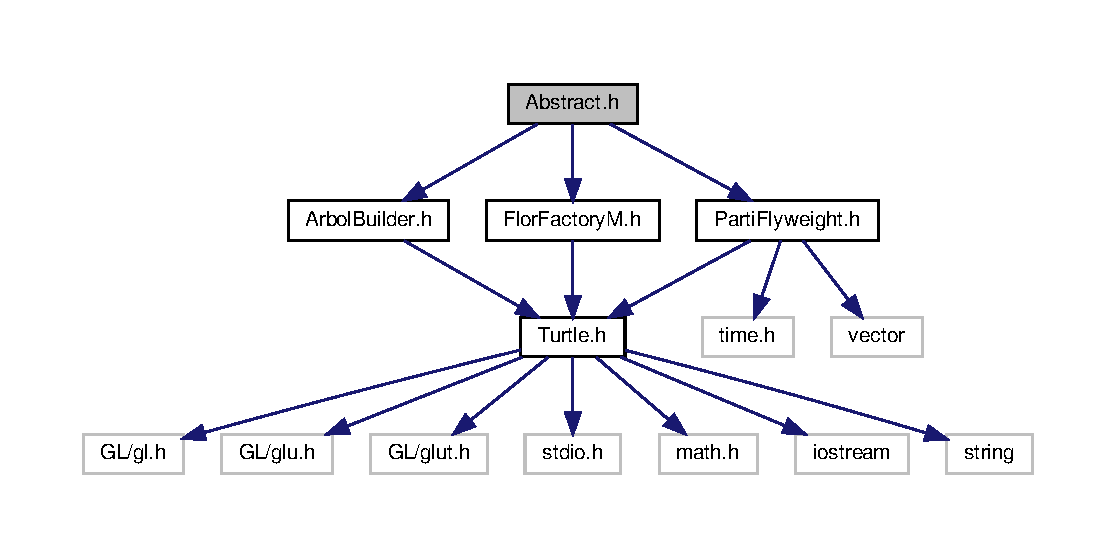
\includegraphics[width=350pt]{Abstract_8h__incl}
\end{center}
\end{figure}
\subsection*{Clases}
\begin{DoxyCompactItemize}
\item 
class \hyperlink{classAbstractFact}{Abstract\+Fact}
\begin{DoxyCompactList}\small\item\em La clase \hyperlink{classAbstractFact}{Abstract\+Fact} contiene funciones virtual-\/pura  Se realiza con funciones virtual-\/pura para que estas sean reutilizadas por nuestras fabricas. \end{DoxyCompactList}\item 
class \hyperlink{classPrim}{Prim}
\begin{DoxyCompactList}\small\item\em La clase \hyperlink{classPrim}{Prim} es la clase \hyperlink{classAbstractFact}{Abstract\+Fact} concreta  Se instancian punteros a cada uno de nuestros objetos. \end{DoxyCompactList}\item 
class \hyperlink{classSeco}{Seco}
\begin{DoxyCompactList}\small\item\em La clase \hyperlink{classSeco}{Seco} es la clase \hyperlink{classAbstractFact}{Abstract\+Fact} concreta  Se instancian punteros a cada uno de nuestros objetos pero esta vez de otro tipo. \end{DoxyCompactList}\end{DoxyCompactItemize}


\subsection{Descripción detallada}
implementacion de la clase \hyperlink{classAbstractFact}{Abstract\+Fact} con el uso de Open\+Gl en C++. 

\begin{DoxyAuthor}{Autor}
i\+Mawe 
\end{DoxyAuthor}
\begin{DoxyVersion}{Versión}
Revision 1.\+1 
\end{DoxyVersion}

\hypertarget{ArbolBuilder_8h}{}\section{Referencia del Archivo Arbol\+Builder.\+h}
\label{ArbolBuilder_8h}\index{Arbol\+Builder.\+h@{Arbol\+Builder.\+h}}


implementacion de la clase \hyperlink{classTreeBuil}{Tree\+Buil} con el uso de Open\+Gl en C++.  


{\ttfamily \#include \char`\"{}Turtle.\+h\char`\"{}}\newline
Dependencia gráfica adjunta para Arbol\+Builder.\+h\+:\nopagebreak
\begin{figure}[H]
\begin{center}
\leavevmode
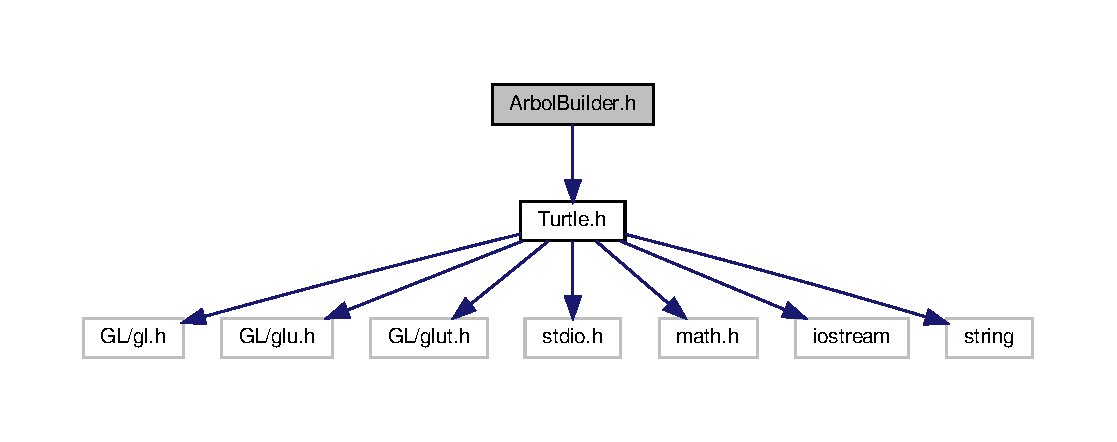
\includegraphics[width=350pt]{ArbolBuilder_8h__incl}
\end{center}
\end{figure}
Gráfico de los archivos que directa o indirectamente incluyen a este archivo\+:\nopagebreak
\begin{figure}[H]
\begin{center}
\leavevmode
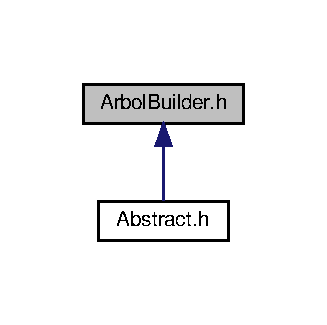
\includegraphics[width=157pt]{ArbolBuilder_8h__dep__incl}
\end{center}
\end{figure}
\subsection*{Clases}
\begin{DoxyCompactItemize}
\item 
class \hyperlink{classTronco}{Tronco}
\begin{DoxyCompactList}\small\item\em La clase \hyperlink{classTronco}{Tronco} contiene la funcion drawn para poder visualizarlo  Se instancia el dato miembro. \end{DoxyCompactList}\item 
class \hyperlink{classHoja}{Hoja}
\begin{DoxyCompactList}\small\item\em La clase \hyperlink{classHoja}{Hoja} contiene la funcion drawn para poder visualizarlo  Se instancia el dato miembro. \end{DoxyCompactList}\item 
class \hyperlink{classRama}{Rama}
\begin{DoxyCompactList}\small\item\em La clase \hyperlink{classRama}{Rama} contiene la funcion drawn para poder visualizarlo  Se instancia el dato miembro. \end{DoxyCompactList}\item 
class \hyperlink{classTree}{Tree}
\begin{DoxyCompactList}\small\item\em La clase \hyperlink{classTree}{Tree} contiene la funcion drawn para visualizar el arbol  Se instancia los datos miembros que son punteros a las partes del arbol. \end{DoxyCompactList}\item 
class \hyperlink{classTreeBuil}{Tree\+Buil}
\begin{DoxyCompactList}\small\item\em La interfaz \hyperlink{classTreeBuil}{Tree\+Buil} contiene las funciones get\+Tronco, get\+Hojas, get\+Ramas para obtener las caracteristicas del arbol  Las funciones son virtual-\/puras y apuntan a las clases de las partes del arbol. \end{DoxyCompactList}\item 
class \hyperlink{classNormalTree}{Normal\+Tree}
\begin{DoxyCompactList}\small\item\em La clase \hyperlink{classNormalTree}{Normal\+Tree} contiene las funciones get\+Tronco, get\+Hojas, get\+Ramas; asi como loset sets de estas para obtener y generar las caracteristicas del arbol  Las funciones apuntan a las clases de las partes del arbol, asi como tambien son void. \end{DoxyCompactList}\item 
class \hyperlink{classDirector}{Director}
\begin{DoxyCompactList}\small\item\em La clase \hyperlink{classDirector}{Director} cse encarga de recolectar todas las caracteristicas para poder formal lo pedido  Utilizando punteros al arbol, se logra enviar la informacion para su elaboracion. \end{DoxyCompactList}\end{DoxyCompactItemize}


\subsection{Descripción detallada}
implementacion de la clase \hyperlink{classTreeBuil}{Tree\+Buil} con el uso de Open\+Gl en C++. 

\begin{DoxyAuthor}{Autor}
i\+Mawe 
\end{DoxyAuthor}
\begin{DoxyVersion}{Versión}
Revision 1.\+1 
\end{DoxyVersion}

\hypertarget{FlorFactoryM_8h}{}\section{Referencia del Archivo Flor\+Factory\+M.\+h}
\label{FlorFactoryM_8h}\index{Flor\+Factory\+M.\+h@{Flor\+Factory\+M.\+h}}


implementacion de la clase \hyperlink{classFlower}{Flower} con el uso de Open\+Gl en C++.  


{\ttfamily \#include \char`\"{}Turtle.\+h\char`\"{}}\newline
Dependencia gráfica adjunta para Flor\+Factory\+M.\+h\+:\nopagebreak
\begin{figure}[H]
\begin{center}
\leavevmode
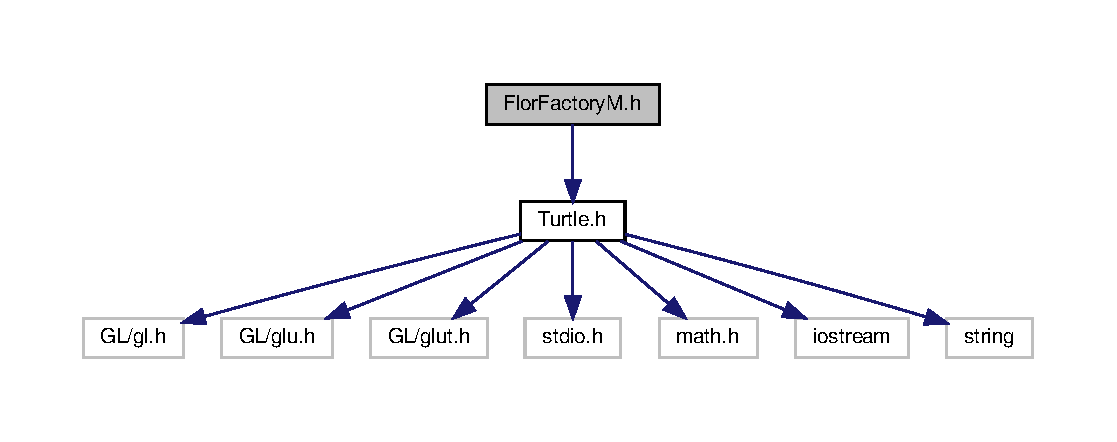
\includegraphics[width=350pt]{FlorFactoryM_8h__incl}
\end{center}
\end{figure}
Gráfico de los archivos que directa o indirectamente incluyen a este archivo\+:\nopagebreak
\begin{figure}[H]
\begin{center}
\leavevmode
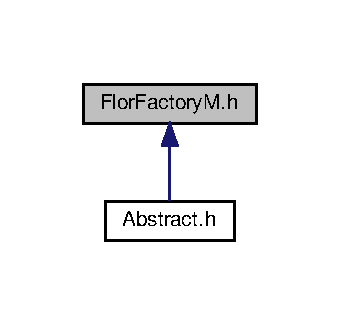
\includegraphics[width=163pt]{FlorFactoryM_8h__dep__incl}
\end{center}
\end{figure}
\subsection*{Clases}
\begin{DoxyCompactItemize}
\item 
class \hyperlink{classFlower}{Flower}
\begin{DoxyCompactList}\small\item\em La clase \hyperlink{classFlower}{Flower} contiene la funcion drawn para poder visualizarlo  Se instancia el dato miembro. \end{DoxyCompactList}\item 
class \hyperlink{classFlorBonita}{Flor\+Bonita}
\begin{DoxyCompactList}\small\item\em La clase \hyperlink{classFlorBonita}{Flor\+Bonita} contiene la funcion drawn para poder visualizarlo, hereda de la clase \hyperlink{classFlower}{Flower}  Se tiene constructor y destructor. \end{DoxyCompactList}\item 
class \hyperlink{classFlorMala}{Flor\+Mala}
\begin{DoxyCompactList}\small\item\em La clase \hyperlink{classFlorMala}{Flor\+Mala} contiene tla funcion drawn para poder visualizarlo, hereda de la clase \hyperlink{classFlower}{Flower}  Se instancia el dato miembro. \end{DoxyCompactList}\item 
class \hyperlink{classFlorNormal}{Flor\+Normal}
\begin{DoxyCompactList}\small\item\em La clase \hyperlink{classFlorNormal}{Flor\+Normal} contiene tla funcion drawn para poder visualizarlo, hereda de la clase \hyperlink{classFlower}{Flower}  Se instancia el dato miembro. \end{DoxyCompactList}\end{DoxyCompactItemize}


\subsection{Descripción detallada}
implementacion de la clase \hyperlink{classFlower}{Flower} con el uso de Open\+Gl en C++. 

\begin{DoxyAuthor}{Autor}
i\+Mawe 
\end{DoxyAuthor}
\begin{DoxyVersion}{Versión}
Revision 1.\+1 
\end{DoxyVersion}

\hypertarget{PartiFlyweight_8h}{}\section{Referencia del Archivo Parti\+Flyweight.\+h}
\label{PartiFlyweight_8h}\index{Parti\+Flyweight.\+h@{Parti\+Flyweight.\+h}}


implementacion de la clase \hyperlink{classSnowFly}{Snow\+Fly} con el uso de Open\+Gl en C++.  


{\ttfamily \#include \char`\"{}Turtle.\+h\char`\"{}}\newline
{\ttfamily \#include $<$time.\+h$>$}\newline
{\ttfamily \#include $<$vector$>$}\newline
Dependencia gráfica adjunta para Parti\+Flyweight.\+h\+:
\nopagebreak
\begin{figure}[H]
\begin{center}
\leavevmode
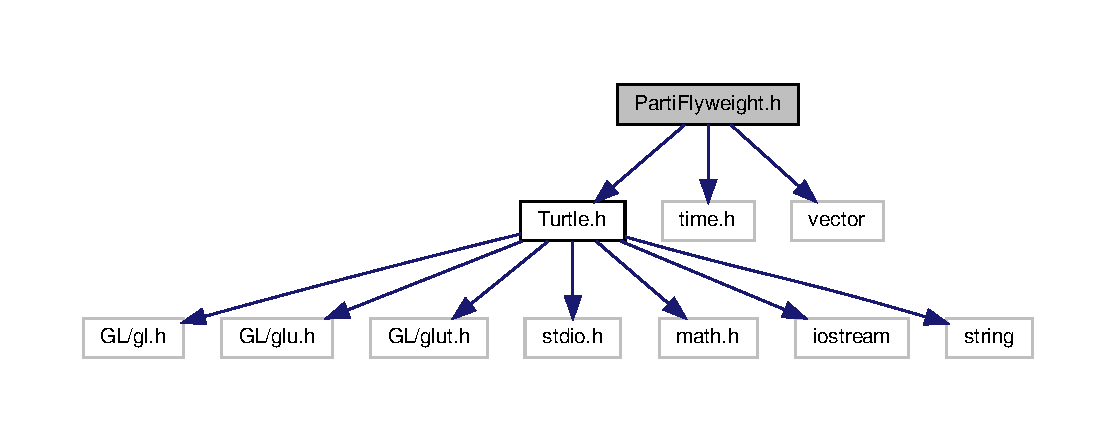
\includegraphics[width=350pt]{PartiFlyweight_8h__incl}
\end{center}
\end{figure}
Gráfico de los archivos que directa o indirectamente incluyen a este archivo\+:
\nopagebreak
\begin{figure}[H]
\begin{center}
\leavevmode
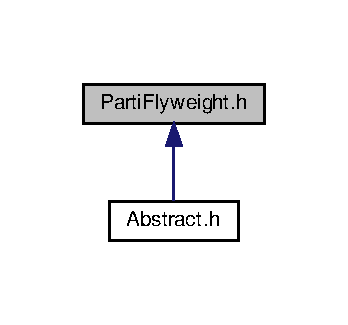
\includegraphics[width=167pt]{PartiFlyweight_8h__dep__incl}
\end{center}
\end{figure}
\subsection*{Clases}
\begin{DoxyCompactItemize}
\item 
class \hyperlink{classSnowFly}{Snow\+Fly}
\begin{DoxyCompactList}\small\item\em La clase \hyperlink{classSnowFly}{Snow\+Fly} contiene las funciones set\+Tam y get\+Tam para poder darle tamano a nuesta nieve  Se instancia el dato miembro tam. \end{DoxyCompactList}\item 
class \hyperlink{classParticle}{Particle}
\begin{DoxyCompactList}\small\item\em La clase \hyperlink{classParticle}{Particle} contiene las funciones display para poder visualizarlo, set cant y gv  Se instancia el dato miembro para cantidad y gv para los pixels que recorre por iteracion. \end{DoxyCompactList}\item 
class \hyperlink{classSnow}{Snow}
\begin{DoxyCompactList}\small\item\em La clase \hyperlink{classSnow}{Snow} contiene las funciones display para poder visualizarlo, set cant y gv  Se instancia el dato miembro para cantidad, gv para los pixels que recorre por iteracion, un vector de particulas para guardar las que son pedidas por el usuario. \end{DoxyCompactList}\end{DoxyCompactItemize}


\subsection{Descripción detallada}
implementacion de la clase \hyperlink{classSnowFly}{Snow\+Fly} con el uso de Open\+Gl en C++. 

\begin{DoxyAuthor}{Autor}
i\+Mawe 
\end{DoxyAuthor}
\begin{DoxyVersion}{Versión}
Revision 1.\+1 
\end{DoxyVersion}

\hypertarget{Turtle_8h}{}\section{Referencia del Archivo Turtle.\+h}
\label{Turtle_8h}\index{Turtle.\+h@{Turtle.\+h}}


implementacion de la clase \hyperlink{classTurtle}{Turtle} con el uso de Open\+Gl en C++.  


{\ttfamily \#include $<$G\+L/gl.\+h$>$}\newline
{\ttfamily \#include $<$G\+L/glu.\+h$>$}\newline
{\ttfamily \#include $<$G\+L/glut.\+h$>$}\newline
{\ttfamily \#include $<$stdio.\+h$>$}\newline
{\ttfamily \#include $<$math.\+h$>$}\newline
{\ttfamily \#include $<$iostream$>$}\newline
{\ttfamily \#include $<$string$>$}\newline
Dependencia gráfica adjunta para Turtle.\+h\+:\nopagebreak
\begin{figure}[H]
\begin{center}
\leavevmode
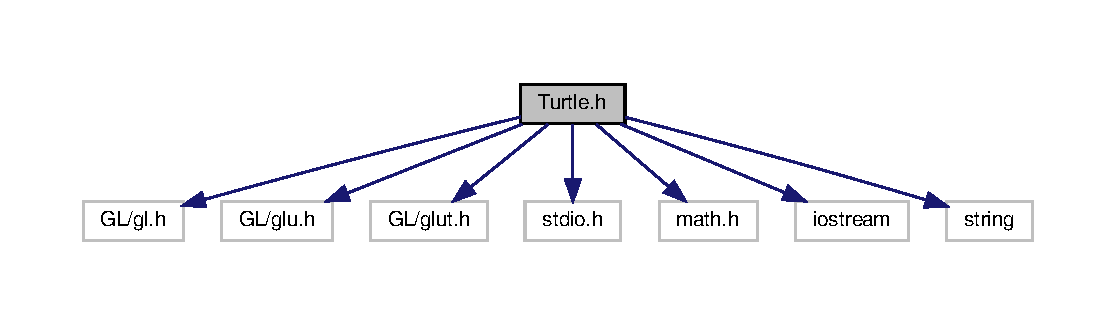
\includegraphics[width=350pt]{Turtle_8h__incl}
\end{center}
\end{figure}
Gráfico de los archivos que directa o indirectamente incluyen a este archivo\+:\nopagebreak
\begin{figure}[H]
\begin{center}
\leavevmode
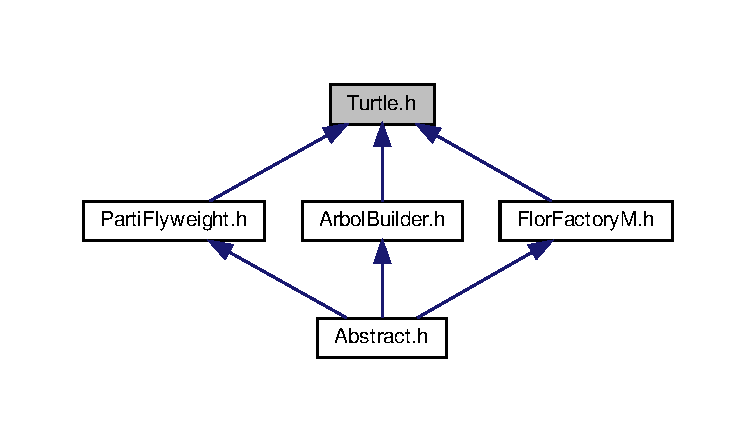
\includegraphics[width=350pt]{Turtle_8h__dep__incl}
\end{center}
\end{figure}
\subsection*{Clases}
\begin{DoxyCompactItemize}
\item 
struct \hyperlink{structCoord}{Coord}
\item 
class \hyperlink{classTurtle}{Turtle}
\begin{DoxyCompactList}\small\item\em La clase tortuga contiene todos los metodos y funciones de \char`\"{}turtle\char`\"{} de Python  Una numeracion general sobre los metodos mas importantes de \char`\"{}turle\char`\"{}. \end{DoxyCompactList}\end{DoxyCompactItemize}
\subsection*{defines}
\begin{DoxyCompactItemize}
\item 
\mbox{\Hypertarget{Turtle_8h_a598a3330b3c21701223ee0ca14316eca}\label{Turtle_8h_a598a3330b3c21701223ee0ca14316eca}} 
\#define {\bfseries PI}~3.\+14159265358979323846
\end{DoxyCompactItemize}


\subsection{Descripción detallada}
implementacion de la clase \hyperlink{classTurtle}{Turtle} con el uso de Open\+Gl en C++. 

\begin{DoxyAuthor}{Autor}
i\+Mawe 
\end{DoxyAuthor}
\begin{DoxyVersion}{Versión}
Revision 1.\+1 
\end{DoxyVersion}

%--- End generated contents ---

% Index
\backmatter
\newpage
\phantomsection
\clearemptydoublepage
\addcontentsline{toc}{chapter}{Índice}
\printindex

\end{document}
